
\NeedsTeXFormat{LaTeX2e}[1995/12/01]
\ProvidesFile{ubcsample.tex}[2012/04/07 v1.70 ^^J
 University of British Columbia Sample Thesis]

\documentclass[msc,oneside]{ubcthesis}
\usepackage{afterpage}
\usepackage{float}
\usepackage{longtable}
\usepackage{graphicx}
\usepackage{pdflscape}
\usepackage[numbers,sort&compress]{natbib}
\usepackage{psfrag}

\usepackage{amsmath}
\usepackage{amsfonts}
\usepackage{graphicx}
\usepackage{nicefrac}
\usepackage{graphicx}
\usepackage{caption}
% \usepackage{subcaption}
\usepackage{subfigure}
% \usepackage{algorithm}
% \usepackage{paralist}
% % \usepackage[geometry]{ifsym}
\usepackage{rotating}
\DeclareMathAlphabet{\mathpzc}{OT1}{pzc}{m}{it}
% \usepackage[normalem]{ulem}
% \usepackage{cite}
% \usepackage{nicefrac}
% % \usepackage{algpseudocode}
\usepackage{varwidth}
\usepackage[linewidth=1pt]{mdframed}
\usepackage{lipsum}
% \usepackage{hyperref}

\usepackage[unicode=true,
  linktocpage,
  linkbordercolor={0.5 0.5 1},
  citebordercolor={0.5 1 0.5},
  linkcolor=blue]{hyperref}

\institution{The University Of British Columbia}

\faculty{The Faculty of Graduate Studies}
\institutionaddress{Vancouver}

\previousdegree{M.Sci., The University of Birmingham, 2012}

% \title{A mixed Finite Element approach to the Magnetohydrodynamics problem}
\title{title}
% \subtitle{With a Subtitle}
\author{Michael Wathen}
\copyrightyear{2014}
\submitdate{\monthname\ \number\year} % The "\ " is required after
                                      % \monthname to prevent the
                                      % command from eating the space.
\program{Computer Science}

\renewcommand\thepart         {\Roman{part}}
\renewcommand\thechapter      {\arabic{chapter}}
\renewcommand\thesection      {\thechapter.\arabic{section}}
\renewcommand\thesubsection   {\thesection.\arabic{subsection}}
\renewcommand\thesubsubsection{\thesubsection.\arabic{subsubsection}}
\renewcommand\theparagraph    {\thesubsubsection.\arabic{paragraph}}
\renewcommand\thesubparagraph {\theparagraph.\arabic{subparagraph}}

\setcounter{tocdepth}{2}
\setcounter{secnumdepth}{2}

\floatstyle{ruled}
\newfloat{Program}{htbp}{lop}[chapter]

% Here is the start of the document.
\sloppy                 % makes TeX less fussy about line breaking

\pagestyle{plain}           % use just a plain page number

\numberwithin{equation}{chapter}    % add the section number to the equation label
\usepackage{amsthm}

\newtheorem{mydef}{Definition}

\usepackage{fancyheadings}

\newcommand{\com}[1]{\texttt{#1}}
\newcommand{\DIV}{\ensuremath{\mathop{\mathbf{DIV}}}}
\newcommand{\GRAD}{\ensuremath{\mathop{\mathbf{GRAD}}}}
\newcommand{\CURL}{\ensuremath{\mathop{\mathbf{CURL}}}}
\newcommand{\CURLt}{\ensuremath{\mathop{\overline{\mathbf{CURL}}}}}
\newcommand{\nullspace}{\ensuremath{\mathop{\mathrm{null}}}}


\newcommand{\FrameboxA}[2][]{#2}
\newcommand{\Framebox}[1][]{\FrameboxA}
\newcommand{\Fbox}[1]{#1}

%\usepackage[round]{natbib}

\newcommand{\half}{\mbox{\small \(\frac{1}{2}\)}}
\newcommand{\hf}{{\frac 12}}
\newcommand {\HH}  { {\bf H} }
\newcommand{\hH}{\widehat{H}}
\newcommand{\hL}{\widehat{L}}
\newcommand{\bmath}[1]{\mbox{\bf #1}}
\newcommand{\hhat}[1]{\stackrel{\scriptstyle \wedge}{#1}}
\newcommand{\R}{{\rm I\!R}}
\newcommand {\D} {{\vec{D}}}
\newcommand {\sg}{{\hsigma}}
%\renewcommand{\vec}[1]{\ensuremath{\mathbf{#1}}}
\newcommand{\E}{\vec{E}}
\renewcommand{\H}{\vec{H}}
\newcommand{\J}{\vec{J}}
\newcommand{\dd}{d^{\rm obs}}
\newcommand{\F}{\vec{F}}
% \newcommand{\C}{\vec{C}}
\newcommand{\s}{\vec{s}}
\newcommand{\N}{\vec{N}}
\newcommand{\M}{\vec{M}}
\newcommand{\A}{\vec{A}}
\newcommand{\B}{\vec{B}}
\newcommand{\w}{\vec{w}}
\newcommand{\nn}{\vec{n}}
\newcommand{\cA}{{\cal A}}
\newcommand{\cQ}{{\cal Q}}
\newcommand{\cR}{{\cal R}}
\newcommand{\cG}{{\cal G}}
\newcommand{\cW}{{\cal W}}
\newcommand{\hsig}{\hat \sigma}
\newcommand{\hJ}{\hat \J}
\newcommand{\hbeta}{\widehat \beta}
\newcommand{\lam}{\lambda}
\newcommand{\dt}{\delta t}
\newcommand{\kp}{\kappa}
\newcommand {\lag} { {\cal L}}
\newcommand{\zero}{\vec{0}}
\newcommand{\Hr}{H_{red}}
\newcommand{\Mr}{M_{red}}
\newcommand{\mr}{m_{ref}}
\newcommand{\thet}{\ensuremath{\mbox{\boldmath $\theta$}}}
\newcommand{\curl}{\ensuremath{\nabla\times\,}}
\renewcommand{\div}{\nabla\cdot\,}
\newcommand{\grad}{\ensuremath{\nabla}}
\newcommand{\dm}{\delta m}
\newcommand{\gradh}{\ensuremath{\nabla}_h}
\newcommand{\divh}{\nabla_h\cdot\,}
\newcommand{\curlh}{\ensuremath{\nabla_h\times\,}}
\newcommand{\curlht}{\ensuremath{\nabla_h^T\times\,}}
\newcommand{\Q}{\vec{Q}}
\renewcommand{\J}{\vec J}
\renewcommand{\J}{\vec J}
% \newcommand{\U}{\vec u}
\newcommand{\V}{\vec v}
\newcommand{\Bt}{B^{\mbox{\tiny{T}}}}
\newcommand{\me}{Maxwell's equations }
\newcommand{\ns}{Navier-Stokes Equations }
\renewcommand{\s}{Stokes Equations }
\newcommand{\Fs}{\vec{f}_{\mbox{\tiny s}}}
\newcommand{\partialt}[1]{\frac{\partial #1}{\partial t}}
\newcommand{\cref}[1]{(\ref{#1})}
% \newcommand{\Ct}{\ensuremath{C^{\mbox{\tiny{T}}}}
\newcommand{\Ct}{\ensuremath{C^{\mbox{\tiny{T}}}}}
\renewcommand{\R}{\mathbb{R}}
\renewcommand{\C}{\mathbb{C}}
\newcommand{\lstPython}[1]{\lstinline[language=Python,breaklines=true,mathescape,literate={\-}{}{0\discretionary{-}{}{}}]§#1§}
\newcommand{\code}[1]{{\ttfamily{#1}}}
\newcommand{\fenics}{FEniCS }
\newcommand{\uu}[1]{\boldsymbol #1}
\renewcommand{\eqref}[1]{(\ref{#1})}
\newcommand{\nedelec}{N\'{e}d\'{e}lec }
\usepackage{setspace}
\usepackage{amsthm}
\newtheorem{prop}{Proposition}[section]
\usepackage{etoolbox}
\usepackage{minted}
\usepackage{zref-xr}
% \AtBeginEnvironment{minted}{\singlespacing}
% \AfterEndEnvironment{minted}{\doublespacing}
% \BeforeBeginEnvironment{minted}{\begin{singlespacing*}}
% \AfterEndEnvironment{minted}{\end{singlespacing*}}
\doublespacing
\usepackage{listings}
\begin{document}
\lstset{language=Python}
% \definecolor{champagne}{rgb}{0.97, 0.91, 0.81}
\newminted{python}{frame=single,mathescape=true,numbersep=11pt,linenos=true}

\definecolor{keywords}{RGB}{255,0,90}
\definecolor{comments}{RGB}{0,0,113}
\definecolor{red}{RGB}{160,0,0}
\definecolor{green}{RGB}{0,150,0}




%% This starts numbering in Roman numerals as required for the thesis
%% style and is mandatory.
\frontmatter


\maketitle                      %% Mandatory
\begin{abstract}                %% Mandatory -  maximum 350 words

\end{abstract}

\chapter{Preface}



\tableofcontents                %% Mandatory
\listoftables                   %% Mandatory if thesis has tables
\listoffigures                  %% Mandatory if thesis has figures

% \chapter{Acknowledgements}      %% Optional

% \chapter{Dedication} %% Optional

\mainmatter
\pagenumbering{arabic}
\setcounter{page}{1}

\chapter{Introduction}

The primary topic of this thesis is to develop and numerically test a large scale implementation of an incompressible magnetohydrodynamics model. In this introductory chapter, we will first  present a description of the model problem studied. We then give a brief overview of finite element methods and Krylov subspace methods for this problem. Finally, we outline the objectives, contributions and structure of the thesis.

\section{A model problem in incompressible magnetohydrodynamics}

The area of incompressible magnetohydrodynamics (MHD)  describes the behaviour of electrically conductive incompressible fluids (liquid metals, plasma, salt water, etc) in an electromagnetic field \cite{davidson2001introduction,le2006mathematical,muller2001magnetofluiddynamics}. MHD models couple electromagnetism and fluid dynamics. The coupling effects are due to two fundamental physical properties. Firstly, through the movement of the conductive material that induces a magnetic field which then modifies any existing electromagnetic field. Secondly, the magnetic and electric fields generate a mechanical force on the fluid known as the Lorentz force. The Lorentz force accelerates the fluid particles in the direction normal to both the electric and magnetic fields.

Incompressible MHD has a number of important applications within technology and industry as well as Geophysical and Astrophysical applications. Some such applications are: electromagnetic pumping, aluminium electrolysis, the Earth's molten core and solar flares. For more applications see \cite{muller2001magnetofluiddynamics}.

In this thesis, we are principally interested in an incompressible MHD model. This means that the electrically conductive fluid is incompressible, i.e., the mass of the fluid is conserved, and the electric resistivity of the fluid cannot be ignored. The MHD model we consider consist of two coupled fundamental equations: the incompressible Navier-Stokes equations and Maxwell's equations. We will outline the derivation of a formulation of an incompressible MHD model for a homogeneous and isotropic medium to ensure that all material parameters are constant; for full details see \cite{armero1996long}.

The transient incompressible Navier-Stokes equations that govern incompressible fluid flow are given by:
\begin{subequations}
\label{eq:ns}
\begin{alignat}2
\rho_f\bigg(\frac{\partial \uu{u}}{\partial t}+ (\uu{u} \cdot \nabla)\uu{u}\bigg)- \mu  \, \Delta\uu{u} +\nabla p &= \uu{f}+\uu{f}_L & \qquad &\mbox{in $\Omega\times(0,T)$},\\[.1cm]
\nabla\cdot\uu{u} &= 0 & \qquad &\mbox{in $\Omega\times(0,T)$}.
\end{alignat}
\end{subequations}
Here $\uu{u}$ and $p$ are the velocity and pressure of the fluid, $\uu{f}$ denotes the body forces acting on the fluid and $\uu{f}_L$ is the Lorentz force, which will be specified later. The parameters $\mu>0$  and $\rho_f>0$ denote the dynamic viscosity and density of the fluid, respectively. The spatial domain is given by $\Omega$ and the end time is denoted by $T$. Mass conservation is given by (\ref{eq:ns}b), see  \cite[Chapter 0]{elman2005finite} for the derivation of the incompressible Navier-Stokes equations.


Maxwell's equations that govern electromagnetic effects are given by:
\begin{subequations}
\label{eq:maxwell2}
    \begin{alignat}2
        &\mbox{Faraday's law:}\quad \quad & \partialt{\uu{b}} +\curl \uu{e} &= \uu{0}, \\
        &\mbox{Coulomb's law:}\quad \quad & \div \uu{d} &= \hat{\rho_{e}}, \\
        &\mbox{Amp\`{e}re's law:}\quad \quad & -\partialt{\uu{d}} + \curl \uu{h} &= {\uu{j}},\\
        &\mbox{Gauss's law:}\quad \quad & \div \uu{b} &= 0.
    \end{alignat}
\end{subequations}
The fields in \eqref{eq:maxwell2} are given by: $\uu{h}$ the magnetic field, $\uu{e}$ the electric field, $\uu{d}$ the electric displacement, $\uu{b}$ the magnetic induction and ${\uu{j}}$ the electric current density. The parameter $\hat{\rho_{e}}$ \RE{is} the electric charge density. In a homogeneous and isotropic medium, the following linear relations hold:
\begin{equation} \label{eq:assumpt}
    \uu{d} = \delta \uu{e}, \quad \uu{b} = \mu \uu{h},
\end{equation}
where the constant $\delta>0$ denotes the electric permittivity and the constant $\mu>0$ the magnetic permeability. Using \eqref{eq:maxwell2} together with \eqref{eq:assumpt} yields the form of Maxwell's equations considered in this thesis:
\begin{subequations}
\label{eq:maxwell}
    \begin{alignat}2
        &\mbox{Faraday's law:}\quad \quad & \partialt{\uu{b}} +\curl \uu{e} &= \uu{0}, \\
        &\mbox{Coulomb's law:}\quad \quad & \div \uu{e} &= \rho_{e}, \\
        &\mbox{Amp\`{e}re's law:}\quad \quad & -\partialt{(\delta\uu{ e})} + \curl (\frac{1}{\mu}\uu{b}) &= \uu{j},\\
        &\mbox{Gauss's law:}\quad \quad & \div \uu{b} &= 0,
    \end{alignat}
\end{subequations}
where $\rho_{e}=\frac{\hat{\rho_{e}}}{\delta}$; see \cite[Chapter 1]{monk2003finite} for more details on Maxwell's equations.


The physical assumptions we consider to form a MHD model are the same as in \cite[Section 2.1]{armero1996long}. More precisely we assume:
\begin{itemize}
    \item Non-relativistic motion: The characteristic fluid velocity is assumed to be orders of magnitude smaller than the speed of light.
    \item Low-frequency approximation: Phenomena involving high frequencies are omitted. That is, the term $\partialt{(\delta\uu{ e})}$ involving the  displacement current is neglected in Maxwell's equations. Therefore, Amp\`{e}re's law~(\ref{eq:maxwell}c) simplifies to
    \begin{equation} \label{eq:AmpereModified}
        \curl \left(\frac{1}{\mu}\uu{b}\right) = \uu{j}.
    \end{equation}
    \item Quasi-neutrality assumption:  Positive and negative charges are equal in any given region. The convection current is omitted and Ohm's law now reads
    \begin{equation} \label{eq:QNassumpt}
        \uu{j} = \theta (\uu{e}+\uu{u}\times\uu{b}),
    \end{equation}
    where positive parameter $\theta$ defines the electric conductivity of the fluid and $\uu{u}\times\uu{b}$ corresponds to the charge density induced by the fluid motion. The electrical resistivity is given by $\nicefrac{1}{\theta}$ and causes dissipative effects in Maxwell's equations but is not to be neglected in this model.
    \item Non-magnetisation and non-polarisation: The assumptions of homogeneity and isotropy also imply that the medium is non-magnetisable and non-polarisable.
\end{itemize}
The Lorentz force $\uu{f}_L$ in (\ref{eq:ns}a) can now be expressed as:
\begin{equation} \label{eq:lorentz}
    \uu{f}_L = \frac{1}{\rho_{f}\,\mu} (\curl \uu{b})\times \uu{b}.
\end{equation}
The electromotive term in \eqref{eq:QNassumpt} now enters Faraday's law (\ref{eq:maxwell}a) by combining \eqref{eq:QNassumpt} and \eqref{eq:AmpereModified} into the following expression for $\uu{e}$:
\begin{equation} \nonumber
    \uu{e} = \frac{1}{\theta}\left(\curl \left(\frac{1}{\mu}\uu{b}\right)-\uu{u}\times\uu{b}\right).
\end{equation}

% \begin{itemize}
%     \item Non-relativistic motion:~\\ In general,  Maxwell's equations are invariant under transformations of the Lorentz group. In this thesis, we assume non-relativistic motion, i.e., the fluid velocity is orders of magnitude smaller than the speed of light. Hence, we assume the Galilean invariant approximation of the electromagnetic field transformations. Defining $\uu{e}'$ and $\uu{b}'$ as the electric field and  magnetic induction at rest in the reference frame  moving at velocity $\uu{u}$ with respect to spatial system, then we suppose that
%     $$\uu{e}'= \uu{e}+\uu{u}\times \uu{b}, \quad \uu{b}'=\uu{b},$$
%     where $\uu{e}$ and $\uu{b}$ are the spatial electric field and spatial magnetic induction.
%     \item High frequencies: ~\\ Phenomena involving high frequencies are not considered, hence, displacement current $\partialt{(\delta\uu{ e})}$ can be neglected. Therefore, Amp\`{e}re's law~(\ref{eq:maxwell}c) simplifies to
%     \begin{equation} \label{eq:AmpereModified}
%         \curl (\frac{1}{\mu}\uu{b}) = \uu{j}.
%     \end{equation}
%     \item Quasi-neutrality: ~\\ Positive and negative charges are equal in any given region. Hence, the convection current can be omitted and Ohm's law becomes
%     $$\uu{j} = \theta \uu{e}'=  \theta (\uu{e}+\uu{u}\times\uu{b}).$$
%     The positive parameter $\theta$ defines the electric conductivity of the fluid and $\uu{u}\times\uu{b}$ describes the flow of the fluid that has been induced by the electric field.  The electrical resistivity is given by $\nicefrac{1}{\theta}$ and causes dissipative effects in Maxwell's equations but is not neglected.
%     \item Non-magnetisable and non-polarised medium: ~\\ This assumption implies that the relations \eqref{eq:assumpt} hold for all values of the electric permeability and magnetic permittivity. Therefore, the Lorentz force $\uu{f}_L$ in (\ref{eq:ns}a) is now given by:
%     $$\uu{f}_L = \frac{1}{\rho_{f}} \uu{j}\times \uu{b}.$$
%     Substituting Amp\`{e}re's law \eqref{eq:AmpereModified} (under the low frequency assumption) into the Lorentz force gives the following relationship:
%     $$\uu{f}_L = \frac{1}{\rho_{f}\,\mu} (\curl \uu{b})\times \uu{b}.$$
% \end{itemize}

{Using the assumptions above, elimination of the electric field $\uu{e}$ and non-dimensionalisation, the systems in \eqref{eq:ns} and \eqref{eq:maxwell} are coupled into the following set of partial differential equations:}
\begin{subequations}
\label{eq:mhdnon}
\begin{alignat}2
 \frac{\partial \uu{u}}{\partial t}- \nu  \, \Delta \uu{u} + (\uu{u} \cdot \nabla) \uu{u}+\nabla p - \kappa\, (\nabla\times\uu{b})\times\uu{b} &= \uu{f}, \\
\nabla\cdot\uu{u} &= 0, \\
\frac{\partial \uu{b}}{\partial t}+\nu_m  \, \nabla\times( \nabla\times \uu{b})
-  \, \nabla\times(\uu{u}\times \uu{b}) &= \uu{0}, \\
\nabla\cdot\uu{b} &= 0,
\end{alignat}
\end{subequations}
 with suitable initial conditions and boundary conditions; see \cite[Section 2]{armero1996long}. The unknowns $\uu{u}$, $p$ and $\uu{b}$ are the fluid velocity, the fluid pressure and the magnetic field, respectively.
 % The first coupling term $\kappa\, (\nabla\times\uu{b})\times\uu{b}$ in (\ref{eq:mhdnon}a) represents to the Lorentz force $f_L$ in \eqref{eq:lorentz}, whereas the second coupling term $\nabla\times(\uu{u}\times \uu{b})$ in (\ref{eq:mhdnon}c) corresponds to the electromotive force modifying the magnetic field, due to the motion of the conductive fluid.


The solution to \eqref{eq:mhdnon} depends on three non-dimensional parameters $\nu = \nicefrac{1}{\rm Re}$, $\nu_m = \nicefrac{1}{\rm Rm}$ and $\kappa$. The first parameter Re is the hydrodynamic Reynolds number, which indicates the balance between the inertial forces and the viscous forces. The parameter Rm is the magnetic Reynolds number, which measures the effect by which the magnetic field induces flow motion. The final parameter, the coupling number, $\kappa$, represents the influence of the electromagnetic field on the flow. It is sometimes defined in terms of the Hartmann number denoted by Ha, as
\begin{equation}
    \nonumber
    \mbox{Ha} = \sqrt{\kappa \, \mbox{Re\,Rm}}.
    % \kappa = \frac{\mbox{Ha}^2}{\mbox{Re\,Rm}}.
\end{equation}
To find typical physical values for these parameters, we refer to \cite{armero1996long,le2006mathematical,roberts1967introduction}. We refer to $\nu$ as the viscosity for the rest of this thesis.

In this thesis, we are interested in the steady-state ($\frac{\partial}{\partial t} = 0$) version of~\eqref{eq:mhdnon}:
\begin{subequations}
\label{eq:steadystate}
\begin{alignat}2
 - \nu  \, \Delta \uu{u} + (\uu{u} \cdot \nabla) \uu{u}+\nabla p - \kappa\, (\nabla\times\uu{b})\times\uu{b} &= \uu{f}, \\
\nabla\cdot\uu{u} &= 0, \\
\label{eq:curlcurl}
\kappa\nu_m  \, \nabla\times( \nabla\times \uu{b})
- \kappa \, \nabla\times(\uu{u}\times \uu{b}) &= \uu{0}, \\
\nabla\cdot\uu{b} &= 0.
\end{alignat}
\end{subequations}
Note we have multiplied (\ref{eq:steadystate}c) by $\kappa$ to enforce skew-symmetry of the coupling terms. We will consider both two- and three-dimensional solutions to \eqref{eq:steadystate}. \RE{See Appendix~\ref{Curl} for curl definitions.}

% The curl operator is well defined in three-dimensions and the two-dimensional curl may be defined as follows: given 2D vector fields $\uu{b}(x,y) = (b_1,b_2)$, $\uu{u}(x,y) = (u_1,u_2)$ and the scalar function $r(x,y)$ then the curl and cross products are
% \begin{subequations}
% \nonumber
% \begin{alignat}2
% \curl \uu{b} &=& \frac{\partial b_2}{\partial x} - \frac{\partial b_1}{\partial y}, \\
% \curl r &=& \Big(\frac{\partial r}{\partial y}, -\frac{\partial r}{\partial x}\Big),\\
% \uu{u} \times \uu{b} &=& u_1b_2-u_2b_1.
% \end{alignat}
% \end{subequations}
% Note that taking the curl of a 2D vector field results in a scalar function which is the component in the normal direction to the 2D field ($z$-component).

\section{Numerical solution}

The partial differential equation (PDE) system given in \eqref{eq:steadystate} requires a numerical approximation as in general an analytical solution is not possible. There are two main components in computing a numerical solution of a PDE:
\begin{itemize}
    \item[1.] Discretisation: take a continuous model and transfer it into a discrete model;
    \item[2.] Solve: take the discretised model and solve for the unknowns.
\end{itemize}
In this thesis, we use mixed finite element methods for discretising an MHD model problem, and solve it using preconditioned Krylov subspace methods.
In the sequel, we briefly describe these components in the context of the approach we take.


\subsection{Finite element methods for incompressible MHD problems}

There are several finite element methods for discretising MHD problems as in \eqref{eq:steadystate}. A common approach in the literature is to approximate the magnetic field using standard nodal $H^1$-conforming elements \cite{phillips2014block,armero1996long,gerbeau2000stabilized,gunzburger1991existence}. Such a formulation enables one to use the following vector calculus identity
\begin{equation} \label{eq:CurlIdentity}
-\Delta \uu{b} = \curl (\curl \uu{b}) - \nabla(\div \uu{b}).
\end{equation}
Since $\uu{b}$ is divergences-free it is then possible to apply an augmentation technique to replace the curl-curl operator with a vector Laplacian. This then reduces one of the principal  computational difficulties, namely the large null-space of the curl-curl operator in \eqref{eq:curlcurl}. However, one of the main problems using $H^1$-conforming elements for the magnetic field is that for non-convex domains (such as the 2D L-shaped domain with a reentrant corner, or the 3D Fichera corner domain with reentrant edges and corners) the magnetic field will converge to a solution that is not correct around the singular point, see \cite{codina2006stabilized,costabel2000singularities}. Therefore, we consider a mixed discretisation that captures singular solutions correctly. One such family of elements are $H({\rm curl})$ conforming \nedelec elements \cite{nedelec1980mixed}.

To enable the use of \nedelec elements for the magnetic field we use the mixed formulation in \cite{schotzau2004mixed,GreifLiSchotzauWei2010}. This leads to the following governing equations in a domain $\Omega$:
\begin{subequations}
\label{eq:mhd}
\begin{alignat}2
\label{eq:mhd1} - \nu  \, \Delta\uu{u} + (\uu{u} \cdot \nabla)
\uu{u}+\nabla p - \kappa\,
(\nabla\times\uu{b})\times\uu{b} &= \uu{f} & \qquad &\mbox{in $\Omega$},\\[.1cm]
\label{eq:mhd2}
\nabla\cdot\uu{u} &= 0 & \qquad &\mbox{in $\Omega$},\\[.1cm]
\label{eq:mhd3}
\kappa\nu_m  \, \nabla\times( \nabla\times \uu{b})
+ \nabla r
- \kappa \, \nabla\times(\uu{u}\times \uu{b}) &= \uu{g} & \qquad &\mbox{in $\Omega$},\\[.1cm]
\label{eq:mhd4} \nabla\cdot\uu{b} &= 0 & \qquad &\mbox{in $\Omega$},
\end{alignat}
\end{subequations}
where we have introduced the Lagrange multiplier, $r$, in the form of $\nabla r$ in \eqref{eq:mhd3}. Again, $\uu{u}$ and $p$ are the velocity and pressure of the fluids and $\uu{b}$ is the magnetic field. The introduction of the Lagrange multiplier, $r$, corresponds to the divergence-free constraint \eqref{eq:mhd4} of the magnetic field. With the addition of the Lagrange multiplier, $r$, we may also introduce a generic forcing term $\uu{g}$ associated with the Maxwell part of \eqref{eq:mhd}.

The numerical tests that we will consider will have inhomogeneous Dirichlet boundary conditions for the fluid and magnetic fields and homogeneous Dirichlet boundary condition for the multiplier, $r$, of the form:
\begin{subequations}
\label{eq:bc}
\begin{alignat}2
\label{eq:bc1} \uu{u} &= \uu{u_D} & \qquad &\mbox{on $\partial\Omega$},\\[.1cm]
\label{eq:bc2}
   \uu{n}\times\uu{b} &= \uu{n} \times \uu{b_D} & \qquad &\mbox{on $\partial\Omega$},\\[.1cm]
\label{eq:bc3}      r &=0 &\qquad &\mbox{on $\partial\Omega$},
\end{alignat}
\end{subequations}
where $\uu{u_D}$ and $\uu{b_D}$ are given functions, and $\uu{n}$ is the unit outward normal to the boundary $\partial \Omega$. Notice, by taking the divergence of equation \eqref{eq:mhd3} we obtain Poisson's equation (as $\div \curl \uu{b} = 0$):
$$\Delta r = \div \uu{g} \quad \mbox{in } \Omega, \quad r = 0 \quad \mbox{on } \partial \Omega.$$
In many physical applications $\uu{g}$ is divergence-free, which implies that the multiplier, $r$, is zero. In general, the main purpose of the magnetic multiplier is to provide stability, see~\cite{demkowicz1998modeling}.




\subsection{Preconditioning incompressible MHD problems}

Incompressible  MHD problems have been extensively studied in the context of various discretisation and formulations. However, the development of preconditioned iterative solutions to MHD problems is limited. \RE{We refer the reader to the Appendix for a review of Krylov subspace solvers for linear systems. In this thesis our focus will be on the implementation of preconditioners which are tailored to MHD model problem.}

% there does not seem to have been much study of preconditioned iterative solutions.

In the literature there have not been too many approaches to precoditioning the MHD equations given in either the non-multiplier form \eqref{eq:steadystate} or with the multiplier form \eqref{eq:mhd}. In the very recent work \cite{phillips2014block}, an operator-based preconditioner for the non-multiplier MHD equations \eqref{eq:steadystate} has been proposed in the context of $H^1$-conforming elements for the magnetic field. To form their preconditioner the authors use the identity \eqref{eq:CurlIdentity} and a discrete commutator idea to form approximations to the Schur complements. This is based on an approach for a preconditioner to the  Navier-Stokes system as in \cite[Chapter 8]{elman2005finite}. The preconditioners  we employ are based on similar Navier-Stokes preconditioners but rely on the Maxwell preconditioner in \cite{greif2007preconditioners} for $H({\rm curl})$ elements.


\section{Objectives and contributions}

The aim of this thesis is to develop and test fully scalable iterative solution methods for the incompressible MHD model \eqref{eq:mhd}, \eqref{eq:bc} using natural Taylor-Hood elements \cite{taylor1973numerical} for the fluid variables and \nedelec mixed element  \cite{nedelec1980mixed} pair for the magnetic variables.  Our numerical results show good scalability with respect to the mesh size. We provide  several tests  to study the performance of the preconditioners with respect to the relevant non-dimensional parameters. We also present two- and three-dimensional results.

To enable large scale preconditioned tests of the MHD model we use the finite element software \fenics \cite{wells2012automated} together with the linear algebra software from {\tt PETSc} \cite{petsc-web-page,petsc-user-ref}. Using these two principal software packages, experiments were run in excess of 20 million degrees of freedom. As well, it provides an example of how significant physical problems described by partial differential equations can be solved by combining state of the art numerical software packages. The aim is to release the code for public use.

As stated above,  little has been done in terms of preconditioned iterations for the MHD model other than the works of  \cite{phillips2014block} for the non-multiplier form \eqref{eq:steadystate}. Our approach is based on $H({\rm curl})$ elements for the magnetic field \cite{schotzau2004mixed}, and motivated by the preliminary results of \cite{li2010numerical} in the context of exactly divergence-free elements for the velocity field. It combines preconditioners for the incompressible Navier-Stokes and Maxwell's equations in \cite{elman2005finite,greif2007preconditioners,MR2911387}.


% The scalable solvers considered in this thesis may now enable more investigation of the physical problems they describe.
The availability of our large-scale solvers and code will hopefully allow more development and research into such MHD models.

\section{Outline}

This thesis is made up of five chapters and is structured as follows. In Chapter 2, we introduce a mixed finite element approximation to the MHD system \eqref{eq:mhd}-\eqref{eq:bc}. The mixed approximation is based on a standard nodal Taylor-Hood finite element approximation for the velocity field and the pressure, together with a mixed \nedelec element approximation for the magnetic field and the multiplier. Using this approximation, we introduce three possible non-linear iteration schemes.

In Chapter 3, we present an overview of the preconditioning approaches for the individual subproblems separately, namely the incompressible Navier-Stokes and Maxwell's equations. We then apply these preconditioning techniques to propose preconditoning strategies for the linearisations which arise from the three non-linear iteration schemes from Chapter~2. In particular, for the coupled linearised Picard scheme we propose an inner-outer preconditioning approach.

In Chapter 4, to perform numerical experiments in both two and three spatial dimensions we use the following two main software packages \fenics \cite{wells2012automated} and {\tt PETSc} \cite{petsc-web-page,petsc-user-ref}. We show convergence results for the linearised MHD system along with the incompressible Navier-Stokes and Maxwell subproblems in isolation. Along with the convergence results we numerically test the preconditioning approaches for the three non-linear iteration schemes, providing heuristic tests with respect to the dimensionless parameters ($\nu$,~$\nu_m$~and~$\kappa$;~see~\eqref{eq:mhd}) and mesh size. These tests examine the robustness of both the preconditioners and the iteration schemes.

Chapter 5 provides conclusions and outlines possible extensions for future work.

% \chapter{FEniCS}

The \fenics project started in 2003 and the aim was create software that automates a finite element discretisation and solution of differential equations. The core libraries used within \fenics are DOLFIN \cite{LoggWells2010a,LoggWellsEtAl2012a}, FFC \cite{KirbyLogg2006a,LoggOlgaardEtAl2012a,OlgaardWells2010b}, FIAT \cite{Kirby2012a,Kirby2004a}, Instant, UFC \cite{AlnaesLoggEtAl2009a,AlnaesLoggEtAl2012a} and UFL \cite{AlnaesEtAl2012,Alnaes2012a}. Along the these core packages \fenics has a few extra optional packages that can be found here \url{http://fenicsproject.org/applications/}.

\section{Overview}

One of the key ideas of \fenics was to be able to write an easy to use software package for the solution of partial differential equations (PDEs). The main underlying code base for \fenics is written in C++. and Python


\fenics supports large range of a different finite element function space. Thus allowing \fenics to be used from electromagnetic problems to fluid. The full list of support elements can be found in table~\ref{tab:FunctionSpace}.
\begin{table}[h!]
    \begin{center}
        \begin{tabular}{ l  l }
            Name    &Usage\\
            \hline
            Argyris*    &``ARG''\\
            Arnold-Winther* &``AW''\\
            Brezzi-Douglas-Fortin-Marini*   &``BDFM''\\
            Brezzi-Douglas-Marini   &``BDM''\\
            Bubble  &``B''\\
            Crouzeix-Raviart    &``CR''\\
            Discontinuous Lagrange  &``DG''\\
            Hermite*    &``HER''\\
            Lagrange    &``CG''\\
            Mardal-Tai-Winther* &``MTW''\\
            Morley* &``MOR''\\
            Nedelec 1st kind H(curl)    &``N1curl''\\
            Nedelec 2nd kind H(curl)    &``N2curl''\\
            Quadrature  &``Q''\\
            Raviart-Thomas  &``RT''
        \end{tabular}
        \caption{Avaliable finite element function space (*only partly supported)}
        \label{tab:FunctionSpace}
    \end{center}
\end{table}



This breath introduction to \fenics will go through how to set up a very simple test case, namely the Poisson equation. For this simple problem we will consider both Dirichlet and Neumann boundary conditions and show how to set up the PDE in its variational form.


\section{Poisson example}

For a simple example to see how FEniCS works consider the Poisson equation. Defining $\Omega \subset \R^n$ to be the domain and the boundary as $\partial \Omega = \Gamma_D \cup \Gamma_N$ where $\Gamma_D$ and $\Gamma_N$ correspond to the Dirichlet and Neumann boundaries respectively. Thus, the Poisson equation with corresponding boundary conditions reads as:
\begin{equation} \label{eq:poisson}
 \left. \begin{aligned}
-\Delta u &= f \quad \mbox{in } \Omega\\
 u &= 0 \quad \mbox{in } \Gamma_D\\
\nabla u \cdot n &= g \quad \mbox{in } \Gamma_N
    \end{aligned}
 \right.
 \qquad \text{}
\end{equation}
For this example we will be considering the following function, domains and boundaries to be:
\begin{itemize}
\item $f = (x-\nicefrac{1}{2})^2-4(y-\nicefrac{1}{2})^4$
\item $g = 5x$
\item $\Omega = [0,1]\times[0,1]$
\item $\Gamma_D = \{(0,y) \cup (1,y) \quad | \quad  0\leq y\leq 1\}$
\item $\Gamma_N = \{(x,0) \cup (x,1) \quad | \quad  0\leq x\leq 1\}$
\end{itemize}
Defining the following trial and test function spaces  $\mathcal{V}$ and $\bar{\mathcal{V}}$ as
\begin{equation} \label{eq:PoissonFuncSpace}
 \left. \begin{aligned}
    \mathcal{V}&=H^1_{u_0}(\Omega)=\left\{\,{u}\in H^1(\Omega)\,:\,\text{${u}=u_{0}$ on $\partial\Omega$}\,\right\}, \\
    \bar{\mathcal{V}}&=H^1_0(\Omega)=\left\{\,{u}\in H^1(\Omega)\,:\,\text{${u}={0}$ on $\partial\Omega$}\,\right\}.
 \end{aligned}
 \right.
 \qquad \text{}
\end{equation}
Thus the variational formulation of (\ref{eq:poisson}) depends on finding $u \in \mathcal{V}$ such that
\begin{equation}
\label{eq:PoissonWeak}a(u,v) = L(v) \quad \forall v\in\bar{\mathcal{V}},
\end{equation}
where
\begin{equation}
a(u,v) = \int_{\Omega} \nabla u \cdot \nabla v \, dx \quad \mbox{and} \quad L(v) = \int_{\Omega} fv dx +\int_{\Gamma_N}gv\,ds.
\end{equation}

\subsection{Defining mesh and function space}

For this example we want to consider a uniform unit square mesh. This is created by using the following python code
\begin{pythoncode}
mesh = UnitSquareMesh(32,32)
\end{pythoncode}
Once the mesh is create we no turn to the function space. For this model problem we want to consider the function space $\mathcal{V}$  and $\bar{\mathcal{V}}$ defined by \eqref{eq:PoissonFuncSpace}. Therefore, the discrete finite element space use is the following space
$$\uu{V}_h  = \{\, \uu{u}\in H_1( \Omega)\, :\, \uu{u}|_K \in {\mathcal P}_{1}(K), \, K \in{\mathcal T}_h \, \},$$
where ${\mathcal T}_h=\{K\}$ regular and quasi-uniform triangles. This function space is create in \fenics using the following command
\begin{pythoncode}
V = FunctionSpace(mesh,'CG',1)
\end{pythoncode}

\subsection{Defining subdomains}
Separating different parts of the boundary is easily done within FEniCS. For this our simple Possion model the boundary is split up into two parts. The top and bottom defines the Dirichlet boundary condition whilst the left and right portions of the boundary define the Neumann conditions. Before partitioning the domain into the Dirichlet and Neumann boundaries we need to define the different sections of the boundary. This is done using classes as follows:
\begin{pythoncode}
# Defining boundary classes
class Left(SubDomain):
    def inside(self, x, on_boundary):
        return near(x[0], 0.0)

class Right(SubDomain):
    def inside(self, x, on_boundary):
        return near(x[0], 1.0)

class Bottom(SubDomain):
    def inside(self, x, on_boundary):
        return near(x[1], 0.0)

class Top(SubDomain):
    def inside(self, x, on_boundary):
        return near(x[1], 1.0)

# Initialize sub-domain instances
left = Left()
top = Top()
right = Right()
bottom = Bottom()
\end{pythoncode}
Using the classes above we group the Dirichlet and Neumann boundaries together. These can then be used to set up the boundary conditions for our problem.
\begin{pythoncode}
boundaries = FacetFunction("size_t", mesh)
boundaries.set_all(0)
left.mark(boundaries, 1)
right.mark(boundaries, 1)
top.mark(boundaries, 2)
bottom.mark(boundaries, 2)
\end{pythoncode}

\subsection{Boundary Conditions and weak formulation}

The boundaries have been split into their separate domains so now we can think about defining the boundary conditions, bilinear and linear (\ref{eq:PoissonWeak}) forms.

First consider the homogeneous Dirichlet boundary:
$$  u = 0 \quad \mbox{in } \Gamma_D.$$
The Dirichlet boundary condition is created by using the  \code{DirichletBC} class. When defining Dirichlet boundary conditions on separate subdomains we need to use four inputs to the  \code{DirichletBC} class. The first one is the function space that the boundary condition applies to, the value on the boundary and then the last two arguments define which part of the boundary the boundary condition is defined on.
\begin{pythoncode}
u0 = Constant(0.0)
bc = DirichletBC(V, u0, boundaries,1)
\end{pythoncode}

To define the variational form of the problem we first need to determine the trial function  \code{u} and test function  \code{v} belonging to the function space $\mathcal{V}$. Furthermore, the source term $f$ and Neumann condition $g$ are required in the linear form $L(v)$. Both are defined using the  \code{Expression} class. Together with the trial and test functions the variational form can be created using the following code:
\begin{pythoncode}
# Define variational problem
u = TrialFunction(V)
v = TestFunction(V)
f = Expression("(pow(x[0]-0.5,2)-4*pow(x[1]-0.5,4))")
g = Expression("(5*x[0])")
a = inner(grad(u), grad(v))*dx
L = f*v*dx + g*v*ds(2)
\end{pythoncode}


\subsection{Assembly and solving}

Now the variational  (or weak form) have been stated the next step is to solve the problem. This can be done in two was within FEniCS
\begin{itemize}
    \item[1.] Assemble system and solve
    \item[2.] Solve without assembly.
\end{itemize}
First, consider assembling then solve the system. This can be done by using the {\code{assemble\_system}} class. This class takes the variational form as the inputs and the Dirichlet boundary condition.
\begin{pythoncode}
A, b = assemble_system(a,L,bc)
\end{pythoncode}
The final solving step is the same for both ways. To do this we first define a function {\code{u}} in the corresponding function space ($\mathcal{V}$) that will represent the solution. Next, calling the \code{solve} function with either the matrix \code{A} and vector \code{b} as the arguments or the variational form will compute the solution using sparse direct solvers which is the  default solving method for \fenics
\begin{pythoncode}
u = Function(V)
solve(A,u.vector(),b)
solve(a == L, u, bc)
\end{pythoncode}

\subsubsection{Optional solution parameters}

For simplicity above the \code{solve} used \fenics default parameters. However, this may not necessarily be the most efficient so may want to change these parameters. It is well known for example that multigrid is the most efficient solve for the Poisson problem. Here is how to set this up.
\begin{pythoncode}
solve(a == L, u, bc,
            solver_parameters=dict(linear_solver="cg",
            preconditioner="amg"))
\end{pythoncode}
For more optional parameters use the following commands:
\begin{pythoncode}
print list_krylov_solver_methods()
print list_krylov_solver_preconditioners()
print list_linear_algebra_backends()
print list_linear_solver_methods()
print list_lu_solver_methods()
\end{pythoncode}

Instead of using FEniCS's inbuilt solving function you can use other external packages. For instance you can link you your FEniCS code with Trilinos \cite{Trilinos-Users-Guide,Trilinos-Overview}, PETSc \cite{petsc-web-page,petsc-user-ref} or your own code.

\subsection{Visualisation}

Once you have solved your problem the next step is to either visualise or save the result. To output the solution in a VTK file you need to create a file with \code{.pvd} suffix. This enables you to use external software (for example ParaView \cite{}) to visualise the solution. Alternatively FEniCS's has an interface for the VTK visualisation tools. We do this by using the \code{plot} command.
\begin{pythoncode}
# Save solution in VTK format
file = File("poisson.pvd")
file << u

# Plot solution
plot(u, interactive=True)
\end{pythoncode}

\begin{figure}[h!]
  \centering
    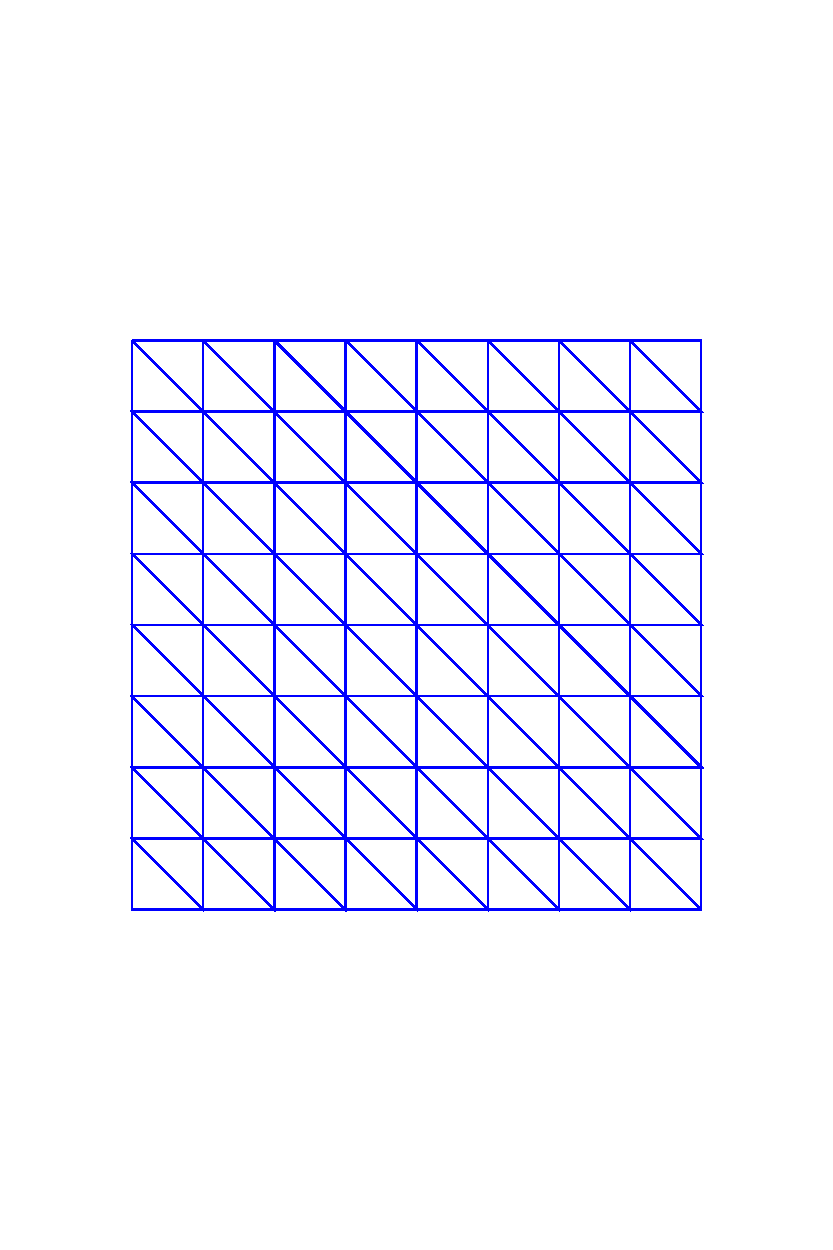
\includegraphics[scale=.6]{../FEniCS/Figures/dolfin_plot_1}
\caption{Numerical solution to (\ref{eq:poisson})}
\end{figure}


% \bibliographystyle{plain}
% \bibliography{/home/mwathen/Dropbox/MastersResearch/MHD/THESIS/ref/ref}


\chapter{Finite element discretisation}
\label{sec:discretization}

In this chapter we introduce a mixed finite element discretisation for the steady-state incompressible MHD problem \eqref{eq:mhd}, \eqref{eq:bc} that models electrically conductive fluids under the influence of a magnetic field.  Following the setting in \cite{schotzau2004mixed}, we use curl-conforming elements for the magnetic field and conforming continuous elements for the velocity field. The resulting discretisation is verified though a series of numerical experiments which appear later in Chapter \ref{chap:results}. For simplicity, we initially only discuss in detail homogeneous Dirichlet boundary conditions, that is
\begin{equation} \label{eq:homogeneousBC}
    \uu{u} = \uu{0} \quad \mbox{and} \quad \uu{n}\times \uu{b} = \uu{0}.
\end{equation}
Inhomogeneous conditions as in \eqref{eq:bc}  are  discussed in Section~\ref{sec:bcig}.


\section{Variational formulation}
\label{sec:variation}

\RE{Suppose that the domain $\Omega$ is a Lipschitz domain of $\mathbb{R}^d$ for $d=2,3$.} To express the problem \eqref{eq:mhd}, \eqref{eq:bc} in weak form we follow \cite{schotzau2004mixed} and denote the $L^2$-inner product on $L^2(\Omega)^d$ by $(\cdot,\cdot)_\Omega$, for $d = 2,3$. We introduce the standard Sobolev spaces
\begin{equation} \label{eq:FuncSpace}
 \left. \begin{aligned}
\hspace{-1.5mm}\uu{V}&=H_0^1(\Omega)^d=\left\{\uu{u}\in H^1(\Omega)^d\,:\,\text{$\uu{u}=\uu{0}$ on $\partial\Omega$}\right\},\\
\hspace{-1.5mm}Q&=L^2_0(\Omega)=\{p\in L^2(\Omega)\,:\,(p\,,1)_\Omega=0\},\\
\hspace{-1.5mm}\uu{C}&=H_0({\rm curl};\Omega) = \left\{\uu{b}\in L^2(\Omega)^d\,:\,\nabla\times\uu{b}\in L^2(\Omega)^{\bar{d}}, \
\text{$\uu{n}\times\uu{b}=\uu{0}$ on $\partial\Omega$}\right\},\\
\hspace{-1.5mm}S&=H^1_0(\Omega)=\{r\in H^1(\Omega)\,:\,r=0\ \mbox{on $\partial\Omega$}\}.
 \end{aligned}
 \right.
 \qquad \text{}
\end{equation}
where $\bar{d}={2d-3}$ is used to cover the 2D and 3D cases. We write $\|\cdot\|_{L^2(\Omega)}$, $\|\cdot\|_{H^1(\Omega)}$ and $\|\cdot\|_{H(\rm{curl};\Omega)}$ for the associated natural norms. More precisely, for  vector fields $\uu{u},\uu{b}$ and a scalar function $r$ the norms are defined as follows:
\begin{equation} \nonumber
 \left. \begin{aligned}
    \|\uu{u}\|_{L^2 (\Omega)} &= \left({\int_{\Omega} \uu{u}\cdot\uu{u}\;dx}\right)^{\frac{1}{2}},\\
   \|\uu{u}\|_{H^1(\Omega)} &=  \left(\|\uu{u}\|_{L^2(\Omega)}^2 + \|\nabla  \uu{u}\|_{L^2(\Omega)}^2 \right)^{\frac{1}{2}},\\
   \|\uu{b}\|_{H(\rm{curl},\Omega)} &=  \left(\|\uu{b}\|_{L^2(\Omega)}^2 + \|\nabla \times \uu{b}\|_{L^2(\Omega)}^2 \right)^{\frac{1}{2}}, \\
    \|r\|_{L^2 (\Omega)} &= \left({\int_{\Omega} r^2\;dx}\right)^{\frac{1}{2}},\\
    \|r\|_{H^1(\Omega)} &=  \left(\|r\|_{L^2(\Omega)}^2 + \|\nabla  r\|_{L^2(\Omega)}^2 \right)^{\frac{1}{2}},\\
 \end{aligned}
 \right.
 \qquad \text{}
\end{equation}
where $\|\nabla  \uu{u}\|_{L^2(\Omega)}^2$ is given by:
$$\|\nabla  \uu{u}\|_{L^2(\Omega)}^2 = \left(\int_{\Omega} \sum^d_{i,j=1}(\nabla \uu{u})_{ij}(\nabla \uu{u})_{ij} \, dx\right)^{\frac12}.$$
The weak formulation of the incompressible MHD system (\ref{eq:mhd}), (\ref{eq:bc}) consists in finding~$(\uu{u},p,\uu{b},r)\in \uu{V} \times Q\times \uu{C} \times S$ such that
\begin{subequations}
\label{eq:weak}
\begin{eqnarray}
\label{eq:weak1} A(\uu{u},\uu{v}) + O(\uu{u};\uu{u},\uu{v})
+C(\uu{b};\uu{v},\uu{b})
+B(\uu{v}, p) & =& (\uu{f}, \uu{v})_{\Omega},\\[.1cm]
\label{eq:weak2}
B(\uu{u},q)&=&0, \\[.1cm]
\label{eq:weak3}
M(\uu{b},\uu{c})-C(\uu{b};\uu{u},\uu{c})+D(\uu{c},r)&=& (\uu{g},\uu{c})_\Omega, \\[.1cm]
\label{eq:weak4} D(\uu{b},s)&=&0,
\end{eqnarray}
\end{subequations}
for all $(\uu{v},q,\uu{c},s)\in \uu{V} \times Q\times \uu{C}\times
S$. The individual variational forms are given by
\begin{equation} \label{eq:forms}
 \left. \begin{aligned}
&A(\uu{u},\uu{v})=  \int_\Omega \nu \, \nabla\uu{u}:
\nabla\uu{v}\,d\uu{x},&\\  & O(\uu{w};\uu{u},\uu{v}) = \int_\Omega
(\uu{w}\cdot\nabla)\uu{u} \cdot\uu{v} \, d\uu{x},
\\[.1cm]
&  B(\uu{u},q) = -\int_\Omega\,(\nabla\cdot\uu{u}) \,q \,d\uu{x},
&\\  &
 M(\uu{b},\uu{c})= \int_\Omega\, \kappa\nu_m
(\nabla\times\uu{b})\cdot(\nabla\times\uu{c})\,d\uu{x},\\[0.1cm]
& D(\uu{b},s) = \int_\Omega\, \uu{b} \cdot \nabla s\,
d\uu{x}, & \\ &
C(\uu{d};\uu{v},\uu{b}) =  \int_\Omega \kappa\, (\uu{v}\times\uu{d})\cdot
(\nabla\times\uu{b})\, d\uu{x},
 \end{aligned}
 \right.
 \quad\text{}
\end{equation}
where  $\nabla \uu{u}:\nabla \uu{v}$ is  defined as
$$\nabla \uu{u}:\nabla \uu{v} = \sum^d_{i,j=1}(\nabla \uu{u})_{ij}(\nabla \uu{v})_{ij}.$$ In \cite{schotzau2004mixed} it has been shown that this formulation of the problem is discretely energy-stable and has a unique solution for small data (i.e. for small $\nu$, $\nu_m$, $\kappa$ and forcing terms $\uu{f}$ and $\uu{g}$ with small $L^2$-norms).

\section{Mixed finite element discretisation}

Consider the domain $\Omega$ to be divided up into a regular and quasi-uniform mesh ${\mathcal T}_h=\{K\}$ consisting of triangles ($d = 2$) or tetrahedra ($d = 3$)  with mesh size $h$. Based on the function spaces defined in \eqref{eq:FuncSpace}, our finite element approximation will be sought in the finite dimensional spaces given by:
\begin{equation}
\label{eq:FiniteSpace}
\begin{split}
\uu{V}_h &=  \{\, \uu{u}\in H^1( \Omega)\, :\, \uu{u}|_K \in {\mathcal P}_{k}(K)^d, \, K \in{\mathcal T}_h \, \},\\[.1cm]
Q_h&=  \{\, p\in L^2(\Omega) \cap H^1(\Omega)\,:\, p|_K \in {\mathcal P}_{k-1}(K), \, K \in{\mathcal T}_h \,\},\\[.1cm]
\uu{C}_h &=  \{\, \uu{b}\in H_0({\rm curl}; \Omega) \,:\, \uu{b}|_K \in {\mathcal P}_{k-1}(K)^d \oplus \uu{R}_k(K), \, K \in{\mathcal T}_h \,\},\\[.1cm]
S_h&=  \{\, r\in H_0^1(\Omega) \,:\, r|_K \in {\mathcal P}_{k}(K), \, K \in {\mathcal T}_h \, \},
\end{split}
\end{equation}
for $k\geq 2$. We define ${\mathcal P}_{k}(K)$ as the space of polynomials of total degree at most $k$ on $K$ and $ \uu{R}_k(K)$ as the space of homogeneous vector polynomials of total degree $k$ on $K$ that are orthogonal to the position vector $\uu{x}$. Here we note that we are using ${\mathcal P_k}/{\mathcal P_{k-1}}$ Taylor-Hood elements for the fluid unknowns $(\uu{u},p)$ \cite{taylor1973numerical}. For the magnetic variables $(\uu{b},r)$ we use the curl-conforming \nedelec element pair     of the first kind \cite{nedelec1980mixed}. These choices of finite elements spaces $\uu{V}_h, \, \uu{C}_h, \, Q_h$ and $S_h$ imply that  we have conforming subspaces to our Sobolev spaces $\uu{V}, \, \uu{C}, \,Q$ and $S$, respectively. Then the finite element solution to \eqref{eq:weak} consists in finding $(\uu{u}_h,p_h,\uu{b}_h,r_h)\in \uu{V}_h\times Q_h\times \uu{C}_h\times S_h$ such that
\begin{subequations}
\label{eq:VariationForm}
\begin{eqnarray}
\label{eq:bn1} \hspace{-15mm} A(\uu{u}_h,\uu{v}) + \tilde{O}(\uu{u}_h;\uu{u}_h,\uu{v}) +C(\uu{b}_h;\uu{v},\uu{b}_h) +B(\uu{v}, p_h) & = & ( \uu{f},\uu{v}),\\[.1cm]
\label{eq:bn2}
B(\uu{u}_h,q)&=& 0, \\[.1cm]
\label{eq:bn3} M(\uu{b}_h,\uu{c})-C(\uu{b}_h;\uu{u}_h,\uu{c})+ D(\uu{c},r_h)&=& (\uu{g},\uu{c}),\\[.1cm]
\label{eq:bn4} D(\uu{b}_h,s)&=&0,
\end{eqnarray}
\end{subequations}
for all $(\uu{v},q,\uu{c},s)\in \uu{V}_h\times Q_h \times \uu{C}_h\times S_h$.

The forms $A, M, B, D$ and $C$ stay the same as on the continuous level. However, for the convection term $\tilde{O}(\cdot;\cdot,\cdot)$ we modify the form $O(\uu{w};\uu{u},\uu{v})$ in a standard fashion to ensure the energy-stability property
\begin{equation} \label{eq:convection}
    \tilde{O}(\uu{w};\uu{u},\uu{u}) = 0, \quad \forall \uu{w},\uu{u} \in  \uu{V}_h.
\end{equation}
To do so we integrate by parts the convection form $O(\uu{w};\uu{u},\uu{u})$  to obtain
\begin{equation} \nonumber
 \left. \begin{aligned}
     \int_\Omega (\uu{w}\cdot\nabla)\uu{u} \cdot\uu{u} \, d\uu{x} =& -\frac{1}{2}\int_{\Omega} \nabla \cdot \uu{w} \uu{u} \cdot \uu{u} \, d\uu{x}
     +\frac{1}{2}\int_{\partial \Omega} \uu{w}\cdot \uu{n} |\uu{u}|^2\, ds,
 \end{aligned}
 \right.
 \qquad \text{}
\end{equation}
recalling that $\uu{n}$ is the unit outward normal on $\partial \Omega$. Therefore, we choose the modified convection form $\tilde{O}(\uu{w};\uu{u},\uu{v})$ as
$$\tilde{O}(\uu{w};\uu{u},\uu{v}) =  \int_\Omega (\uu{w}\cdot\nabla)\uu{u} \cdot\uu{v} \, d\uu{x} +\frac{1}{2}\int_{\Omega} \nabla \cdot \uu{w} \uu{u} \cdot \uu{v}\, d\uu{x}-\frac{1}{2}\int_{\partial \Omega} \uu{w}\cdot \uu{n} \uu{u} \cdot \uu{v}\, ds.$$
By construction, property \eqref{eq:convection} is now satisfied. Note also that for homogeneous boundary conditions as assumed in \eqref{eq:homogeneousBC}, the boundary integral term in $\tilde{O}$ can be omitted.

Again in \cite{schotzau2004mixed} it has been shown that this variational formulation of a MHD problem is discretely energy-stable and has a unique solution for small data. Also, optimal order error estimates in the mesh size $h$ have been derived for small data using the stability property \eqref{eq:convection}. Namely, for sufficiently smooth solutions, we have the error bound
$$\|\uu{u}-\uu{u}_h\|_{H^1(\Omega)}+\|\uu{b}-\uu{b}_h\|_{H(\rm{curl};\Omega)}+\|p-p_h\|_{L^2(\Omega)}+\|r-r_h\|_{H^1(\Omega)} \leq C h^k,$$
for a constant $C>0$ independent of the mesh size. In addition, the $L^2$-norm error for the velocity field is of order $\mathcal{O}(h^{k+1})$ (as $\uu{V}_h$ consists of a full polynomial space on each element). However, we cannot expect $L^2$-norm errors of  order $\mathcal{O}(h^{k+1})$ for the magnetic field (as $\uu{C}_h$ does not consist of a full polynomial space on each element).


\subsection{Matrix representation}

The variational formulation \eqref{eq:VariationForm} now can be converted into a matrix representation. To do this, we introduce the basis function for the finite element spaces in \eqref{eq:FiniteSpace}:
\begin{alignat}2
\label{eq:bases1}
\uu{V}_h & = \mbox{span}\langle  \uu{\psi}_j \rangle _{j=1}^{n_u}, & \qquad &
Q_h  = \mbox{span} \langle  \alpha_i \rangle _{i=1}^{m_u},\\[0.1cm]
 \uu{C}_h& =\mbox{span}\langle \uu{\phi}_j \rangle _{j=1}^{n_b}, & \qquad & S_h = \mbox{span} \langle \beta_i
\rangle_{i=1}^{m_b}.
\end{alignat}
The aim now is to find the coefficient vectors $u = (u_1, \ldots , u_{n_u}) \in \mathbb{R}^{n_u}$, $p = (p_1, \ldots , p_{m_u}) \in \mathbb{R}^{m_u}$, $b = (b_1, \ldots , b_{n_b}) \in \mathbb{R}^{n_b}$, and $r = (r_1, \ldots , r_{m_b}) \in \mathbb{R}^{m_b}$ of the finite element functions $(\uu{u}_h, p_h,\uu{b}_h, r_h)$ in terms of the chosen bases. As usual, this is done by writing the bilinear forms in \eqref{eq:VariationForm} in terms of the following stiffness matrices and load vectors:
\begin{alignat*}2
A_{i,j} &= A(\uu{\psi}_j,\uu{\psi}_i), &\quad  &1 \leq i,j \leq n_u,\\[0.1cm]
B_{i,j} &= B(\uu{\psi}_j,\alpha_i), &\quad &1 \leq i \leq m_u, \ 1 \leq j \leq n_u,\\[.1cm]
D_{i,j} &= D(\uu{\phi}_j,\beta_i),  & & 1 \leq i \leq m_b,\ 1 \leq j \leq n_b,\\[.1cm]
M_{i,j}&= M(\uu{\phi}_j,\uu{\phi}_i), &\qquad & 1 \leq i,j \leq n_b,\\[.1cm]
f_i &= (\uu{f},\uu{\psi}_i)_\Omega, & & 1\leq i\leq n_u,\\[.1cm]
g_i &= (\uu{g},\uu{\phi}_i)_\Omega, & & 1\leq i \leq n_b.
\end{alignat*}
For the two non-linear forms, $\tilde{O}$ and $C$, we define the corresponding stiffness matrices with respect to given finite element functions $\uu{w}_h \in \uu{V}_h$ and $\uu{d}_h\in \uu{C}_h$ in the first argument and their associated coefficient vectors $w$ and $d$ as
\begin{alignat*}2
O(w)_{i,j} &=\tilde{O}(\uu{w}_h;\uu{\psi}_j,\uu{\psi}_i), &\quad  &1 \leq i,j \leq n_u,\\[.1cm]
C(d)_{i,j} &= C(\uu{d}_h;\uu{\psi}_j,\uu{\phi}_i), & & 1\leq i \leq n_b,\ 1 \leq j \leq n_u.
\end{alignat*}

Thus, the numerical solution to \eqref{eq:mhd} consists in solving the non-linear system
\begin{equation}
\label{eq:matrix-system}
\left(
\begin{array}{cccc}
A+O(u) & B^T & C^T(b) & 0\\
B & 0 & 0 & 0\\
-C(b) & 0 & M & D^T \\
0 & 0 & D & 0
\end{array}
\right)
\,
\left(
\begin{array}{c}
u\\
p\\
b\\
r
\end{array}
\right) =
\left(
\begin{array}{c} f\\0\\g\\0
\end{array}
\right),
\end{equation}
where the vectors  $u\in\mathbb{R}^{n_u}$, $p\in\mathbb{R}^{m_u}$,  $b\in\mathbb{R}^{n_b}$, and $r\in\mathbb{R}^{m_b}$ are the unknown coefficients of the finite element functions.

\section{Picard iteration (P)}
\label{sec:nonlinear}
The discrete system \eqref{eq:matrix-system} is non-linear, and therefore appling a non-linear solver to this problem is necessary. A common choice to deal with the non-linearity within the incompressible Navier-Stokes equations in isolation is to perform Oseen or Picard iterations \cite{elman2005finite}. This involves linearising around the current velocity and solving for updates.

% One (at least theoretical) advantage of the discrete Oseen system is that it is provably energy-stable (for the skew-symmetrized form which we use) for all values of nu. That is, the matrix is not symmetric but positive definite, which might be an advantage for preconditioning. For small data (i.e. for large \nu) the fixed-point iteration is a contraction.

\RE{For simplicity we only consider the linearly convergent Picard iterations. Since we have modified the convection form to be discretely energy-stable as in \eqref{eq:convection}, an advantage of this approach is that the discrete convection-diffusion operator is real positive. Thus, with small data the fixed-point/Picard iteration is a contraction. A more efficient non-linear solver is Newton's method which converges quadratically near the solution. However, applying Newton's method is more involved, as it requires construction and solving linear systems associated with a Jacobian as well as finding an initial guess sufficiently close to the solution.
% A common approach to ensure convergence with Newton's method is to perform a few Picard iterations before starting the Newton scheme.
% In Section~5.2 we mention the possibility of using Newton's method as an area of future work.
We leave the implementation of Newton's method or other non-linear solvers as an area of possible future work (Section~5.2).
}

% \RE{For simplicity we only consider the linearly convergent Picard iterations. An example of a more efficient non-linear solver is Newton's method which converges quadratically. However, the main difficulty with Newton's method is that convergence is only local and hence the initial guess needs to be sufficiently accurate to obtain convergence. Since we have modified the convection form to be descretely energy-stable \eqref{eq:convection} then an advantage of the discrete Oseen systems is that the matrix is positive definite. Thus, this provides an advantage for preconditioning and with small data the fixed-point/Picard iterations is a contraction.
% % A common approach to ensure convergence with Newton's method is to perform a few Picard iterations before starting the Newton scheme.
% % In Section~5.2 we mention the possibility of using Newton's method as an area of future work.
% We leave the implementation of Newton's method or other non-linear solvers as an area of possible future work (Section~5.2).
% }

\RE{We adapt the fixed-point/Picard iterations to an approach for the full MHD system, where we linearise around the current velocity and magnetic fields.} Given a current iterate $(\uu{u}_h,p_h,\uu{b}_h,r_h)$  we solve for updates $(\delta \uu{u}_h,\delta p_h,\delta \uu{b}_h,\delta r_h)$ and introduce the next iterate by setting:
\begin{equation}\nonumber
\begin{array}{cc}
% \label{eq:updates}
\uu{u}_h& \hspace{-3mm} \rightarrow \uu{u}_h +\delta \uu{u}_h, \quad p_h \rightarrow p_h +\delta p_h,\\
\uu{b}_h& \hspace{-3mm}  \rightarrow \uu{b}_h +\delta \uu{b}_h, \quad r_h \rightarrow r_h +\delta r_h.
\end{array}
\end{equation}
In variational form, the updates $(\delta \uu{u}_h,\delta p_h,\delta \uu{b}_h,\delta r_h)\in \uu{V}_h\times Q_h \times \uu{C}_h\times S_h$ are found by solving the Picard system (P):
\begin{equation} \nonumber
% \label{eq:picard}
\begin{split}
A(\delta\uu{u}_h, \uu{v}) +\tilde{O}(\uu{u};\delta\uu{u}_h,\uu{v})+ C(\uu{b}_h;\uu{v},\delta \uu{u}_h) + B(\uu{v}, \delta p_h) & = R_u(\uu{u}_h,\uu{b}_h,p_h;\uu{v}),\\[.1cm]
B(\delta\uu{u}_h,q)&= R_p(\uu{u}_h;q), \\[.1cm]
M(\delta \uu{b}_h,\uu{c})+
D(\uu{c},\delta r_h)-C(\uu{b}_h;\delta \uu{u}_h,\uu{v})&= R_b(\uu{u}_h,\uu{b}_h,r_h;\uu{c}),\\[.1cm]
D(\delta \uu{b}_h,s)&= R_r(\uu{b}_h;s),
\end{split}
\end{equation}
for all $(\uu{v},q,\uu{c},s)\in \uu{V}_h\times Q_h \times \uu{C}_h\times S_h$. Note that this system is linearised around $(\uu{u}_h,\uu{b}_h)$. The right-hand side linear forms correspond to the residual at the current iteration $(\uu{u}_h,p_h,\uu{b}_h,r_h)$ defined by:
\begin{align*}
 R_u(\uu{u}_h,\uu{b}_h,p_h;\uu{v})&=(\uu{f}, \uu{v})_\Omega-A(\uu{u}_h,\uu{v})
-  \tilde{O}(\uu{u}_h;\uu{u}_h,\uu{v}) \\  & \hspace{4.2mm}- C(\uu{b}_h;\uu{v},\uu{b}_h)-B(\uu{v},p_h),\\[.1cm]
R_p(\uu{u}_h;q)&=-B(\uu{u}_h,q),\\[.1cm]
 R_b(\uu{u}_h,\uu{b}_h,r_h;\uu{c})&=(\uu{g,c})_\Omega -M(\uu{b}_h,\uu{c})
+ C(\uu{b}_h;\uu{u}_h,\uu{c})-D(\uu{c},r_h),\\[.1cm]
R_r(\uu{b}_h;s)&=-D(\uu{b}_h,s),
\end{align*}
for all $(\uu{v},q,\uu{c},s)\in \uu{V}_h\times Q_h \times \uu{C}_h\times S_h$.

In \cite{schotzau2004mixed} it is shown that for small data the Picard iteration (P) will converge to the exact solution for any initial guess.

To formulate the variational form of the Picard iteration (P) in matrix form, let $({u},p,{b},r)$ be the coefficient vectors associated with $(\uu{u}_h,p_h,\uu{b}_h,r_h)$ and $(\delta{u},\delta p,\delta{b},\delta r)$ be the coefficient vectors of $(\delta \uu{u}_h,\delta p_h,\delta \uu{b}_h,\delta r_h)$. Then it can readily seen that the Picard iteration (P) amounts to solving the matrix system
\begin{equation}
\label{eq:mhd_saddle}
%\mathcal{K} x \equiv
\left(
\begin{array}{cccc}
A+O(u) & B^T & C(b)^T & 0\\
B & 0 & 0 & 0 \\
-C(b) & 0 & M & D^T\\
0 & 0 & D & 0
\end{array}
\right)
\,
\left(
\begin{array}{c}
\delta u\\
\delta p\\
\delta b\\
\delta r
\end{array}
\right)  =
\begin{pmatrix}
r_u \\
r_p\\
r_b\\
r_r
\end{pmatrix},
\end{equation}
with
\begin{equation} \label{eq:rhsupdate}
\begin{array}{rl}
r_u &= f- Au -O(u) u - C(b)^T b- B^T p,\\
r_p &=-B u,\\
r_b &=g-Mu+C(b)b-D^T r,\\
r_r &=-D b.
\end{array}
\end{equation}
At each non-linear iteration, the right hand side vectors and matrices $O(u)$ and $C(b)$ in \eqref{eq:rhsupdate} and \eqref{eq:mhd_saddle} respectively must be assembled with the solution coefficient vectors $({u},p,{b},r)$ of the current iterate. Here, the matrix $A$  is symmetric positive definite (SPD), $O(u)$ is non-symmetric and $-C(b)$, $C(b)^T$ appear in a skew symmetric fashion. We also note that $M$ is symmetric positive semidefinite (SPSD) with nullity $m_b$ corresponding to the dimension of the scalar space $S_h$ giving rise to the discrete gradients, see \cite{greif2007preconditioners}.


\section{Decoupled iterations}
\label{sec:FEMdecouple}


The full MHD system \eqref{eq:mhd}, \eqref{eq:bc} is a coupled system consisting of the incompressible Navier-Stokes and Maxwell's equations, coupled through the non-linear skew symmetric coupling term $C(b)$. In addition, the convection term $O(u)$ is non-linear as well. These two terms make the numerical solution challenging. Therefore, if one or both of these terms is small then it may be possible to iterate explicitly. In particular if the coupling term, $C(b)$, is small then we may completely decouple the system into an incompressible Navier-Stokes problem and a Maxwell problem. The two resulting decoupling schemes are what we call Magnetic and Complete Decoupling and are both described below. Note that unlike the Picard iteration, there is no small data guarantee that such iterations based on these decoupling schemes will converge; although we see convergence for reasonable values of the non-dimensional parameters.


\subsection{Magnetic Decoupling (MD)}
\label{sec:FEMmd}

Consider first the situation where there is  weak coupling within the system, that is when $C(b)$ is small. Then it may be possible to drop these terms to completely decouple the system into the two subproblems, the incompressibleNavier-Stokes and Maxwell's equations. We will call this approach Magnetic Decoupling (MD).
% For a given solution $(\uu{u}_h,p_h,\uu{b}_h,r_h)$, neglecting the coupling terms in \eqref{eq:picard} results in solving for the updates $(\delta \uu{u}_h,\delta p_h,\delta \uu{b}_h,\delta r_h) \in \uu{V}_h \times Q_h \times \uu{C}_h \times S_h$  such that
% \begin{equation}
% \label{eq:picard_explicit_MD}
% \begin{split}
% A(\delta\uu{u}_h, \uu{v}) +O(\uu{u};\delta\uu{u}_h,\uu{v})+ B(\uu{v}, \delta p_h) & = R_u(\uu{u}_h,\uu{b}_h,p_h;\uu{v})\\[.1cm]
% B(\delta\uu{u}_h,q)&= R_p(\uu{u}_h;q), \\[.1cm]
% M(\delta \uu{b}_h,\uu{c})+
% D(\uu{c},\delta r_h)&= R_b(\uu{u}_h,\uu{b}_h,r_h;\uu{c}),\\[.1cm]
% D(\delta \uu{b}_h,s)&=R_r(\uu{b}_h;s),
% \end{split}
% \end{equation}
% where again $(\uu{v},q,\uu{c},s)\in\uu{V}_h\times Q_h\times\uu{C}_h\times S_h$ and $R_u$, $R_p$, $R_b$ and $R_r$ which are defined in section \ref{sec:nonlinear}. Again, let $({u},p,{b},r)$ be the coefficient vectors of $(\uu{u}_h,p_h,\uu{b}_h,r_h)$ and $(\delta{u},\delta p,\delta{b},\delta r)$ be the coefficient vectors of $(\delta \uu{u}_h,\delta p_h,\delta \uu{b}_h,\delta r_h)$, then this amounts to solving the linear system:
Then the system\eqref{eq:mhd_saddle} simplifies to
\begin{equation}
\label{eq:matrix_MD}
%\mathcal{K} x \equiv
\left(
\begin{array}{cccc}
A+O(u) & B^T & 0 & 0\\
B & 0 & 0 & 0 \\
0 & 0 & M & D^T\\
0 & 0 & D & 0
\end{array}
\right)
\,
\left(
\begin{array}{c}
\delta u\\
\delta p\\
\delta b\\
\delta r
\end{array}
\right)  =
\begin{pmatrix}
r_u \\
r_p\\
r_b\\
r_r
\end{pmatrix},
\end{equation}
with
\begin{align*}
r_u &= f- Au -O(u)u - C(b)^T b- B^T p,\\[0.1cm]
r_p &=-B u,\\[0.1cm]
r_b &=g-Mu+C(b)b-D^T r,\\[0.1cm]
r_r &=-D b.
\end{align*}
We iterate in the same fashion as the Picard iteration with the simpler matrix \eqref{eq:matrix_MD}. From \eqref{eq:matrix_MD} we can see that the system is now completely decoupled. This enable us to  solve each individual subproblem separately and possibly in parallel.

\subsection{Complete Decoupling (CD)}
\label{sec:FEMcd}

For the second decoupling scheme, we again consider there to be weak coupling of the system but we also consider that the fluid equations are diffusion-dominated and hence can exclude the convection terms.
% This is the simplest technique as it removes all non-linear terms. Again, for a given solution $(\uu{u}_h,p_h,\uu{b}_h,r_h)$, removing the coupling and convection terms in \eqref{eq:picard} results in solving for the updates $(\delta \uu{u}_h,\delta p_h,\delta \uu{b}_h,\delta r_h) \in \uu{V}_h \times Q_h \times \uu{C}_h \times S_h$  such that
% \begin{equation}
% \label{eq:picard_explicit_CD}
% \begin{split}
% A_h(\delta\uu{u}_h, \uu{v}) + B(\uu{v}, \delta p_h) & = R_u(\uu{u}_h,\uu{b}_h.p_h;\uu{v})\\[.1cm]
% B(\delta\uu{u}_h,q)&= R_p(\uu{u}_h;q), \\[.1cm]
% M(\delta \uu{b}_h,\uu{c})+
% D(\uu{c},\delta r_h)&= R_b(\uu{u}_h,\uu{b}_h,r_h;\uu{c}),\\[.1cm]
% D(\delta \uu{b}_h,s)&=R_r(\uu{b}_h;s),
% \end{split}
% \end{equation}
% where $(\uu{v},q,\uu{c},s)\in\uu{V}_h\times Q_h\times\uu{C}_h\times S_h$.  Taking $({u},p,{b},r)$ as the coefficient vectors of $(\uu{u}_h,p_h,\uu{b}_h,r_h)$ and $(\delta{u},\delta p,\delta{b},\delta r)$ be the coefficient vectors of $(\delta \uu{u}_h,\delta p_h,\delta \uu{b}_h,\delta r_h)$, then the proposed decoupled linear system is
This amounts to the system
\begin{equation}
\label{eq:matrix_CD}
%\mathcal{K} x \equiv
\left(
\begin{array}{cccc}
A & B^T & 0 & 0\\
B & 0 & 0 & 0 \\
0 & 0 & M & D^T\\
0 & 0 & D & 0
\end{array}
\right)
\,
\left(
\begin{array}{c}
\delta u\\
\delta p\\
\delta b\\
\delta r
\end{array}
\right)  =
\begin{pmatrix}
r_u \\
r_p\\
r_b\\
r_r
\end{pmatrix},
\end{equation}
with
\begin{align*}
r_u &= f- Au -O(u)u - C(b)^T b- B^T p,\\[0.1cm]
r_p &=-B u,\\[0.1cm]
r_b &=g-Mu+C(b)b-D^T r,\\[0.1cm]
r_r &=-D b.
\end{align*}
Again, we perform iterations in the same fashion as the Picard iteration. This is the simplest technique as it removes all non-linear terms in the iteration matrix and hence leaves the linear Stokes problem in the upper $(1,1)$ block matrix.

\section{Inhomogeneous Dirichlet boundary conditions and initial guess}
\label{sec:bcig}

% In this section, we described the formulation of the MHD system \eqref{eq:mhd}, \eqref{eq:homogeneousBC}, that is with homogeneous Dirichlet boundary conditions. In general, the problems we numerically test have inhomogeneous Dirichlet boundary conditions \eqref{eq:bc}.

When considering inhomogeneous Dirichlet boundary conditions as in \eqref{eq:bc}, we still solve \eqref{eq:mhd_saddle}, \eqref{eq:matrix_MD} and \eqref{eq:matrix_CD} for the solution updates with homogeneous Dirichlet boundary conditions. Therefore, in this approach we must incorporate the inhomogeneous Dirichlet boundary conditions only within the initial guess.

% To start the non-linear iteration schemes given in Section \ref{sec:FEMdecouple} we require an initial guess.

To form a suitable initial guess, we solve the decoupled Stokes problem with the inhomogeneous boundary condition (\ref{eq:bc}a):
\begin{equation} \label{eq:StokesInitial}
\left(
\begin{array}{cc}
A & B^T \\
B & 0 \\
\end{array}
\right)
\left(
\begin{array}{c}
u \\
p \\
\end{array}
\right)=\left(
\begin{array}{c}
f \\
0 \\
\end{array}
\right),
\end{equation}
and then the non-symmetric Maxwell problem the with inhomogeneous boundary conditions (\ref{eq:bc}b), (\ref{eq:bc}c):
\begin{equation} \label{eq:MaxwellInitial}
\left(
\begin{array}{cc}
M -C(u) & D^T \\
D & 0 \\
\end{array}
\right)
\left(
\begin{array}{c}
b \\
r \\
\end{array}
\right)=\left(
\begin{array}{c}
g \\
0 \\
\end{array}
\right).
\end{equation}
Here the term $C(u)$ corresponds the coupling term using $u$ (the initial guess for the velocity field). We expect the inclusion of the coupling term to increase the accuracy of the initial guess because additional information of the problem is used.


% When iteratively solving these two systems, the convergence tolerance for the initial guess is important.  Since the updates will have homogeneous boundary conditions then the initial guess needs to incorporate the inhomogeneous boundary conditions. Consider for example the fluid equations: if the discrete Stokes problem is solved approximately to some tolerance, then the we approximately solve the boundary equations of the form:
% $$1\times u_B = u_D,$$
% where $u_B$ is the coefficients of the solution on the boundary and $u_D$ is a sufficiently accurate boundary data interpolation. That is that the initial guess only starts with boundary values of the same order of accuracy as the initial solve.


The inhomogeneous Dirichlet boundary conditions are incorporated in a standard fashion by suitably modifying the matrix system. The outcome of this procedure is that the boundary data interpolation is only performed for the initial guess. Hence, the iterative solves for the initial guess must be run to a sufficient accuracy to ensure the accuracy of the discrete boundary conditions.

% If the subsequent solution updates (which have homogeneous Dirichlet boundary conditions) are solver accurately, the inaccuracy in the boundary values will remain. For similar reasons, low accuracy of the solution updates will lead to perturbation in the boundary conditions and thus in the whole solution.


% Suppose you solve for the initial guesses $(u_0,p_0,b_0,r_0,)$ one would get an error associated with the boundary $(\delta u_B,\delta p_B,\delta b_B,\delta r_B)$ so that
% \begin{equation} \nonumber
%  \left. \begin{aligned}
%         u_0 &= u+\delta u_B, & \quad&
%         p_0 = p+\delta p_B,\\
%         b_0 &= b+\delta b_B,  &\quad &
%         r_0 = r+\delta r_B.\\
%  \end{aligned}
%  \right.
%  \qquad \text{}
% \end{equation}
% When $(u_0,p_0,b_0,r_0,)$ as the initial guess and then solving for the updates (which have homogeneous Dirichlet boundary conditions) there will still be some error associated with the boundaries  which are $(\delta u_B,\delta p_B,\delta b_B,\delta r_B)$. This therefore means that if the Stokes and Maxwell solves are not done accurately enough then when solving for the updates errors will remain within the boundary conditions. Thus the error norms for the full MHD system will be capped by the accuracy of the Stokes and Maxwell solves for the initial guess.

%%%%%%%%%%%%%%%%%%%%%%%%%%%%%%%%%%%%%%%%%%%%%%%%%%%%%%%%%%%%%%%%%%%%%%%%%%%%%%%%%%%%%%%%%%%%%%%%%%%%%%%%%%%%%%%%%%%%%%%%%%%%%%%%%%%%%%%%%%%%%%%%%%%%%%%%%%%%%%%%%%%%%%%%%%%%%%%%%%%%%%%%%%%%%%%%%%%%%%%%%%%%%%%%%%%%%%%%%%%%%%%%%%%%%%%%%%%%%%%%%%%%%%%%%%%%%%%%%%%%%%%%%%%%%%%%%%%%%%%%%%%%%%%%%%%%%%%%%%%%%%%%%%%%%%%%%%%%%%%%%%%%%%%%%%%%%%%%%%%%%%%%%%%%%%%%%%%%%%%%%%%%%%%%%%%%%%%%%%%%%%%%%%%%%%%%%%%%%%%%%%%%%%%%%%%%%%%%%%%%%%%%%%%%%%%%%%%%%%%%%%%%%%%%%%%%%%%%%%%%%%%%%%%%%%%%%%%%%%%%%%%%%%%%%%%%%%%%%%%%%%%%%%%%%%%%%%%%%%%%%%%%%%%%%%%%%%%%%%%%%%%%%%%%%%%%%%%%%%%%%%%%%%%%%%%%%%%%%%%%%%%%%%%%%%%%%%%%%%%%%%%%%%%%%%%%%%%%%%%%%

% To start the Picard iterations given in Section \ref{sec:nonlinear} we require an initial guess. To form the initial guess, we solve the decoupled Stokes problem
% $$
% \left(
% \begin{array}{cc}
% A & B^T \\
% B & 0 \\
% \end{array}
% \right)
% \left(
% \begin{array}{c}
% u \\
% p \\
% \end{array}
% \right)=\left(
% \begin{array}{c}
% f \\
% 0 \\
% \end{array}
% \right),
% $$
% then the non-symmetric Maxwell problem
% $$\left(
% \begin{array}{cc}
% M -C & D^T \\
% D & 0 \\
% \end{array}
% \right)
% \left(
% \begin{array}{c}
% b \\
% r \\
% \end{array}
% \right)=\left(
% \begin{array}{c}
% g \\
% 0 \\
% \end{array}
% \right).$$
% Here the term $C$ corresponds the the coupling term using $u$ (the initial guess for the velocity field). We use the coupling term within the non-symmetric Maxwell problem as we have the initial guess for the velocity field and incorporating this into the solve for the magnetic and multiplier fields initial guess will hopefully increase the accuracy of the initial guess.


% When solving these two systems, the convergence tolerance which we use is important. In particular, inaccurate solutions cause problems with non-homogeneous boundary conditions. This is because if the matrix system with the boundary conditions applied is not solve to a sufficient accuracy then there will be errors in the boundary data. When we solved for the updates we enforce homogeneous Dirichlet boundary conditions (i.e., zero boundary conditions) on the velocity ($u$), magnetic ($b$) and multiplier ($r$) fields. This therefore means that if the Stokes and Maxwell solves are not done accurately enough then when solving for the updates errors will remain within the boundary conditions. Thus the error norms for the full MHD system will be capped by the accuracy of the Stokes and Maxwell solves for the initial guess.




\section{Summary}

In this chapter we reviewed a mixed finite element approximation to the full MHD system given in \eqref{eq:mhd} and \eqref{eq:bc}. We followed the mixed approach outlined in \cite{schotzau2004mixed} and expressed the MHD system in the matrix form \eqref{eq:mhd_saddle}. Using the Picard iteration  \eqref{eq:mhd_saddle} we introduced two possible decoupling schemes ((MD) and (CD)) which may be simpler to solve for. The performance of the resulting three non-linear iteration schemes depends on the values of the parameters $\kappa$, $\nu$ and $\nu_m$. The next chapter will discuss possible preconditioning approaches for these systems.

In the sequel, we shall omit the dependence of $O(u)$ and $C(b)$ on $u$ and~$b$, respectively, and simply  write $O$ and $C$.









%  \chapter{Linear Solver}

In many applications one of the main problems is to find the solution of a linear system. This system may arise form an optimisation or, like here, a discretised PDE. In this chapter we will go through the two methods which this is done.

\section{Direct Methods}

Suppose you are given a linear system of the form
$$Ax = b$$
where $A$ is a real $n\times n$ non-singular matrix and right hand side vector $b \in \mathcal{R}^n$, where the aim is to solve for the vector $x \in \mathcal{R}^n$. All direct methods are based on Gaussian elimination.

\subsection{Software}

UMFPACK \cite{Davis:2004:CPS:992200.992205,Davis:2004:AUV:992200.992206,Davis:1999:CUM:305658.287640,davis1997unsymmetric}, PASTIX \cite{henon2002pastix}, SuperLU \cite{superlu_ug99,li05} and MUMPS \cite{amestoy2000multifrontal,amestoy2001fully,amestoy2006hybrid}


\section{Iterative Methods}




\chapter{Preconditioning}
\label{chap:precond}

The linear system \eqref{eq:mhd_saddle} is typically sparse and of large dimensions, hence to efficiently solve for it we use a preconditioned iterative approach as proposed in \cite{li2010numerical}. We start by reviewing some preconditioning strategies for the incompressible Navier-Stokes and Maxwell subproblems in isolation. From these techniques we will then introduce and  numerically test  preconditioners for the full MHD system in linearised form as in \eqref{eq:mhd_saddle}.

Let us introduce a number of matrices in addition to the ones already defined in Chapter~2: the velocity mass matrix $Q$, the pressure mass matrix $Q_p$, the pressure convection diffusion matrix  $F_p$, the pressure Laplacian matrix $A_p$, the scalar Laplacian matrix $L$ and the mass matrix~$X$ by
\begin{subequations}
\label{eq:PrecondMatrices}
\begin{eqnarray}
Q_{i,j}&=&\int_\Omega\, \uu{\psi_j}\cdot \uu{\psi_i} \,d\uu{x}, \quad 1\leq i,j \leq n_u,\\
(Q_p)_{i,j}&=& \int_\Omega\, \alpha_j \alpha_i \,dx, \ \ 1\leq i,j \leq m_u, \\
(F_{p})_{i,j}&=& \nu \int_\Omega\, \grad \alpha_j \cdot \grad \alpha_i +(\uu{w} \cdot \grad \alpha_j)\alpha_i\,dx,\ \ 1\leq i,j \leq m_u, \\
(A_{p})_{i,j}&=&  \int_\Omega\, \grad \alpha_j \cdot \grad \alpha_i \,dx, \ \ 1\leq i,j \leq m_u, \\
L_{i,j}&=&\int_\Omega\,\nabla\beta_j\cdot\nabla\beta_i\,d\uu{x},  \ \ 1\leq i,j \leq m_b\\
X_{i,j}&=&\int_\Omega\, \uu{\phi}_j\cdot\uu{\phi}_i\,d\uu{x},  \ \ 1\leq i,j \leq n_b,
\end{eqnarray}
\end{subequations}
where $\uu{w}$ is the finite element velocity from the current iteration. The matrices $F_p$ and $A_p$ are well defined as we use continuous elements for the pressure finite element space $Q_h$. The matrices incorporate homogeneous Neumann boundary conditions.

\section{Preconditioning the incompressible Navier-Stokes equations}
\label{sec:NSprecond}


Consider the steady state incompressible Navier-Stokes equations in isolation. Let
\begin{equation}
\label{eq:ns_coeff}
\mathcal{K}_{\rm NS}=
\begin{pmatrix}
F & B^T \\
B & 0
\end{pmatrix},
\end{equation}
be the discretised and linearised Navier-Stokes (or Oseen) subproblem where $F~=~A~+~O$ has been defined in \eqref{eq:forms}. Due to the convection term, $O$, this  system is non-symmetric and we will use GMRES to iteratively solve this subproblem; \cite{saad1986gmres}. A common approach for solving a saddle point system, as in \eqref{eq:ns_coeff}, is to use a block diagonal or block triangular preconditioner of the form
\begin{equation}
\label{eq:ns_pc_upper}
\mathcal{M}_{\rm tNS} =
\begin{pmatrix}
F & B^T \\
0 & -S
\end{pmatrix} \quad \mbox{or} \quad
\mathcal{M}_{\rm dNS} =
\begin{pmatrix}
F & 0 \\
0 & S
\end{pmatrix},
\end{equation}
where $S\approx B F^{-1} B^T$ is an approximation to the Schur complement. If $S = B F^{-1} B^T$ is {\em precisely} the Schur complement, then it has been proved in~\cite{murphy2000note} that the preconditioned matrix has exactly $2$ eigenvalues when using the block triangular preconditioner  (i.e., $\mathcal{M}_{\rm tNS}^{-1}\mathcal{K}_{\rm NS}$) or $3$ distinct eigenvalues in the block diagonal case  (i.e., $\mathcal{M}_{\rm dNS}^{-1}\mathcal{K}_{\rm NS}$). Both are diagonalisable and hence GMRES will converge in exactly 2 or 3 iterations in the absence of round-off errors.

In practice it is often too expensive to form and solve for the exact Schur complement $B F^{-1} B^T$, hence, a good approximation is needed. Two well-known preconditioners for the incompressible Navier-Stokes equations are the Least Squares Commutator (LSC) and the Pressure Convection-Diffusion (PCD) preconditioners. A description of both can be found in \cite{elman2005finite} and we will just outline the procedure how these can be applied on the discrete level. For the Navier-Stokes preconditioner we will consider block triangular preconditioners of the same form as $\mathcal{M}_{\rm tNS}$.

% Both methods (LSC and PCD)  start with the convection-diffusion operator associated with the velocity space $\uu{V}_h$ given by
% $$\mathcal{L} = -\nu \Delta +\uu{w} \cdot \nabla\, .$$
% As before $\uu{w}$ is the discrete velocity calculated at the previous non-linear iteration. Suppose that there is a corresponding operator defined in the pressure space
% $$\mathcal{L}_p = (-\nu \Delta +\uu{w} \cdot \nabla)_p\, .$$
% Consider the commutator of the convection-diffusion operator associated with the gradient operator
% \begin{equation} \label{eq:ContCommutator}
% \epsilon = (-\nu \Delta +\uu{w} \cdot \nabla)\nabla - \nabla (-\nu \Delta +\uu{w} \cdot \nabla)_p
% \end{equation}
% to be small. In fact, if $\uu{w}$ was constant then $\epsilon = 0$. We will be using \eqref{eq:ContCommutator} to derive both LSC and PCD.



\subsection{Pressure Convection-Diffusion (PCD)}
\label{sec:PCD_outline}


In \cite[Chap. 8]{elman2005finite} the discrete commutator of the convection-diffusion operator associated with the gradient operation is introduced and given by
\begin{equation} \label{eq:DisCommutator}
    \epsilon_h = (Q^{-1}F)(Q^{-1}B^T)-(Q^{-1}B^T)(Q_p^{-1}F_p).
\end{equation}
where the matrices $Q$, $Q_p$ and $F_p$ are defined in  \eqref{eq:PrecondMatrices}. Assuming that the commutator is small then pre- and post-multiplying \eqref{eq:DisCommutator} by $B F^{-1} Q$ and $F_p^{-1}Q_p$, respectively, let us separate out the Schur complement to give
\begin{equation} \label{eq:SchurApprox}
    BF^{-1}B^T \approx B Q^{-1}B^T F_p^{-1} Q_p.
\end{equation}

Our discretisation is inf-sup stable which implies that there is spectral equivalence between $BQ^{-1}B^T$ and the pressure Laplacian matrix, $A_p$; see \cite[Section 5.5.1]{elman2005finite}. Hence, the Schur complement can be approximated by:
$$S_{\rm PCD} =A_p F_p^{-1}Q_p.$$
Applying the PCD preconditioner (i.e., taking $S = S_{\rm PCD}$) to the linearised Navier-Stokes system involves solving the system
\begin{equation} \nonumber
% \label{eq:matrix-system}
\left(
\begin{array}{cc}
F & B^T \\
0 & -A_p F_p^{-1}Q_p
\end{array}
\right)
\,
\left(
\begin{array}{c}
x \\
y
\end{array}
\right) =
\left(
\begin{array}{c}a\\b
\end{array}
\right)
\end{equation}
at each Krylov iteration. This can be solved  efficiently by splitting it into the following two steps
\begin{itemize} \label{it:PCDsolve}
    \item[1.] Solve for $y$: $y = -Q_p^{-1}F_p A_p^{-1}b;$
    \item[2.] Solve for $x$: $x = F^{-1}(a-B^Ty).$
\end{itemize}
This means that we have one pressure Poisson solve ($A_p^{-1}$), one mass matrix solve ($Q_p^{-1}$), one convection-diffusion solve ($F^{-1}$) and multiplications with $F_p$ and $B^T$ at each Krylov iteration. It is possible to solve these iteratively using multigrid and/or iterative methods. However, to test the preconditioner we will use direct solver in this thesis.

\subsection{Least-Squares Commutator (LSC)}
\label{sec:LSC_outline}

One disadvantage with using the PCD preconditioner is that it requires the construction of the matrices $A_p$, $Q_p$ and $F_p$ in \eqref{eq:PrecondMatrices}. A second approach to approximate the Schur complement is the LSC preconditioner \cite[Chap. 8]{elman2005finite} which primarily uses the available matrix coefficients in \eqref{eq:ns_coeff} and the construction of $Q$ to form the preconditioner (without explicitly forming $A_p$, $Q_p$ and $F_p$).

As for the derivation of the PCD preconditioner we start off with the discrete commutator of the convection-diffusion operator
\begin{equation} \nonumber
    \epsilon_h = (Q^{-1}F)(Q^{-1}B^T)-(Q^{-1}B^T)(Q_p^{-1}F_p).
\end{equation}
Suppose that the $Q$-norm is defined by $\|v\|_{Q} = (Qv,v)^{\nicefrac{1}{2}}$. Then this time we minimise $\epsilon_h$ over the $j$th column of $F_p$ (that is $[F_p]_j$) in the $Q$-norm to try to find an approximation for $F_p$. As shown in \cite{elman2005finite}, the minimisation is given by
$$\min \|[Q^{-1}FQ^{-1}B^T]_j-Q^{-1}B^TQ_p^{-1}[F_p]_j) \|_Q.$$
Solving this optimisation problem, as shown in \cite{elman2005finite}, is done by solving the  normal equations
$$Q_p^{-1}BQ^{-1}B^TQ_p^{-1}F_p = Q_p^{-1}BQ^{-1} FQ^{-1}B^T.$$
This yields the an approximation to $F_p$ as
$$F_p \approx Q_p(BQ^{-1}B^T)^{-1}(BQ^{-1} FQ^{-1}B^T).$$
By substituting this into expression \eqref{eq:SchurApprox} we obtain the LSC approximation to the Schur complement:
\begin{equation} \nonumber
    S \approx BF^{-1}B^T \approx S_{\rm LSC} = (B Q^{-1} B^T)(BQ^{-1}FQ^{-1}B^T)^{-1}(B Q^{-1} B^T).
\end{equation}
Therefore, applying the LSC preconditioner to the Oseen system $\mathcal{K}_{\rm NS}$ in \eqref{eq:ns_coeff} involves solving for the matrix
\begin{equation} \nonumber
\left(
\begin{array}{cc}
F & B^T \\
0 & -S_{\rm LSC}
\end{array}
\right)
\,
\left(
\begin{array}{c}
x \\
y
\end{array}
\right) =
\left(
\begin{array}{c}a\\b
\end{array}
\right)
\end{equation}
at each Krylov iteration. Again, this can be efficiently split up into the following two steps:
\begin{itemize}
    \item[1.] Solve for $y$: $y = -(B Q^{-1} B^T)^{-1}(BQ^{-1}FQ^{-1}B^T)(B Q^{-1} B^T)^{-1}b;$
    \item[2.] Solve for $x$: $x = F^{-1}(a-B^Ty).$
\end{itemize}
Hence, we have two pressure Poisson solves ($(B Q^{-1} B^T)^{-1}$) and one convection-diffusion solve ($F^{-1}$) at each Krylov iteration as well as matrix multiplications. In practice, we take the diagonal or lumped diagonal of $Q$ to form $B Q^{-1} B^T$. These solves, as  with the PCD preconditioner, will be done directly in this thesis.

\subsection{PCD versus LSC}

The main advantage of solving the commutator using the least-squares approach is that the matrices that define the preconditioner are available from the original system $\mathcal{K}_{\rm NS}$ in \eqref{eq:ns_coeff} and the construction of $Q$ . However, for PCD we require the construction of the matrices $A_p$, $Q_p$ and $F_p$. Therefore, LSC is slightly more computationally efficient to form. On the other hand, to apply the LSC preconditioner we require two pressure Poisson solves, whereas PCD only requires one.

We will consider experiments with both preconditioners for the incompressible Navier-Stokes problem in isolation to determine which seems more effective. This preconditioner  will then be applied within the solver for the linearised MHD system.

\section{Preconditioning Maxwell's equations}
\label{sec:MaxwellPrecond}

Next, consider the Maxwell subproblem
\begin{equation}
\label{eq:m_coeff}
\mathcal{K}_{\rm MX}=
\begin{pmatrix}
M & D^T \\
D & 0
\end{pmatrix},
\end{equation}
appearing in a linearised MHD system \eqref{eq:mhd_saddle}.
% , but without coupling terms.
As we did for the Navier-Stokes subproblem in Section \ref{sec:NSprecond}, we apply a block preconditioning strategy for $\mathcal{K}_{\rm MX}$ in  \eqref{eq:m_coeff}. Notice that, $\mathcal{K}_{\rm MX}$ in \eqref{eq:m_coeff} is symmetric and hence we will focus on SPD block diagonal preconditioners.

\subsection{An ideal preconditioner}

The $(1,1)$ block of $\mathcal{K}_{\rm MX}$ is the curl-curl operator, hence, the matrix $M$ is singular, where the null space is of dimension $m_b$ and consists of the discrete gradients. Therefore the usual Schur complement does not exist as the matrix $M$ cannot be inverted. To overcome this difficulty, we employ the approach in  \cite{golub2003solving,greif2006preconditioners} based on  augmentation and use preconditioners of the form:
\begin{equation} \nonumber
% \label{eq:maxwell_pc_ideal}
\begin{pmatrix}
M+D^T W^{-1} D & 0 \\
0 & W
\end{pmatrix},
\end{equation}
where $W$ is a symmetric positive definite matrix.

% . More precisely, we consider replacing $M$ by $M+D^T\mathcal{W}^{-1}D$ where $\mathcal{W}\in {\mathbb R}^{m_b\times m_b}$ is a symmetric positive definite matrix just to form the preconditioner, see \cite{golub2003solving,greif2006preconditioners} for more details. The addition of the matrix ($D^T\mathcal{W}^{-1}D$) removes the singularity of the $(1,1)$ block of $\mathcal{K}_{\rm MX}$ without changing the solution (since $Db = 0$).  In practice, we don't actually replace $M$ by $M+D^T\mathcal{W}^{-1}D$ but just consider preconditioners with $M+D^T\mathcal{W}^{-1}D$ in the $(1,1)$ block which then are applied to $\mathcal{K}_{\rm MX}$. For the Maxwell subproblem the appropriate choice of $\mathcal{W}$ is the scalar Laplacian on $S_h$ defined as $L=(L_{i,j})_{i,j=1}^{m_b} \in{\mathbb R}^{m_b \times m_b}$ with
% \begin{equation}
% \label{eq:scalar_laplace}
% L_{i,j}=\int_\Omega\,\nabla\beta_j\cdot\nabla\beta_i\,d\uu{x},
% \end{equation}
% see  \cite{greif2007preconditioners}. Therefore, the augmented system is given by:
% \begin{equation}
% \label{eq:AugmentMaxwell}
% \bar{\mathcal{K}}_{\rm MX}=
% \begin{pmatrix}
% M + D^TL^{-1}D & D^T \\
% D & 0
% \end{pmatrix}.
% \end{equation}



It has been shown in \cite{greif2007preconditioners} that an appropriate choice of $W$ is the scalar Laplacian, $L$, defined in \eqref{eq:PrecondMatrices}. This leads to the ideal preconditioner:
\begin{equation}
\label{eq:maxwell_pc_ideal}
\mathcal{M}_{\rm iMX} =
\begin{pmatrix}
M+D^T L^{-1} D & 0 \\
0 & L
\end{pmatrix}.
\end{equation}
Applying \eqref{eq:maxwell_pc_ideal} as the preconditioner yields exactly two eigenvalues, $1$ and $-1$ of algebraic multiplicities of $n_b$ and $m_b$, respectively. Therefore using this matrix as a preconditioner means that MINRES will converge in two iterations, in the absence of roundoff errors  \cite{paige1975solution}. However, forming the matrix $M+D^T L^{-1} D$ is costly, hence, $\mathcal{M}_{\rm iMX}$  is  impractical  for large systems.


\subsection{A practical preconditioner}

A good approximation for $M+D^T L^{-1} D$ is required to make the ideal preconditioner, $\mathcal{M}_{\rm iMX}$, suitable in practice. It has been shown in \cite{greif2007preconditioners}  that $M+D^T L^{-1} D$ is spectrally equivalent to $M+X$  where $X$ is the vector mass matrix on the magnetic space defined in \eqref{eq:PrecondMatrices}. Using this approximation yields the practical preconditioner
\begin{equation}
\label{eq:maxwell_pc_X}
\mathcal{M}_{\rm MX} =
\begin{pmatrix}
N& 0 \\
0 & L
\end{pmatrix},
\end{equation}
where $N = M+X$ is a shifted curl-curl operator. A scalable multigrid solver for $N$ has been developed in \cite{hiptmair2007nodal} which involves one shifted Laplacian solves on the vector space and one scalar Laplacian solve. However, the construction of this multigrid solver is involved and hence we will consider direct solves for this preconditioner and leave the multigrid implementation as a possible area of future work.

\section{Preconditioning the MHD equations}
\label{sec:MHDp}
In Section \ref{sec:nonlinear} and \ref{sec:FEMdecouple} we introduced three iteration schemes, namely Picard iteration (P), Magnetic Decoupling (MD) and Complete Decoupling (CD). Using the results from Sections \ref{sec:MaxwellPrecond} and \ref{sec:NSprecond} we will discuss the preconditioning approaches that we apply for these non-linear iteration schemes.


\subsection{Picard iteration}
\label{sec:MHDprecond}

% In Sections \ref{sec:NSprecond} and \ref{sec:MaxwellPrecond} we looked briefly at the preconditioning strategies for the Navier-Stokes and Maxwell's equations.

Using the techniques of Sections \ref{sec:NSprecond} and \ref{sec:MaxwellPrecond} for the incompressible Navier-Stokes and Maxwell problems, respectively, we will look at possible scalable preconditioners for the linearised MHD problem
\begin{equation} \label{eq:K}
    {\mathcal K}_{\rm MH} = \left(
\begin{array}{cccc}
A+O & B^T & C^T & 0\\
B & 0 & 0 & 0\\
-C & 0 & M & D^T \\
0 & 0 & D & 0
\end{array}
\right).
\end{equation}
% Using the Navier-Stokes and Maxwell subproblem preconditioners \eqref{eq:ns_pc_upper} and \eqref{eq:maxwell_pc_X} respectively, then w
We propose the following preconditioner for ${\mathcal K}_{\rm MH}$
\begin{equation}
\label{eq:mhd_pc_ls}
\mathcal{M}_{\rm MH} =
\left(
\begin{array}{cccc}
F & B^T & C^T & 0\\
0 & -{S} & 0 & 0 \\
-C & 0 & N & 0\\
0 & 0 & 0 & L
\end{array}
\right),
\end{equation}
where ${S}$ is now either the LSC or PCD approximation to the fluid flow Schur complement. The preconditioned matrix, $\mathcal{M}_{\rm MH}^{-1}{\mathcal K}_{\rm MH}$, has eigenvalues $\lambda = 1$ with algebraic multiplicity of at least $n_u + n_b$ and the eigenvalue $\lambda = -1$ with algebraic multiplicity of at least $m_b$ see \cite[Theorem~8]{li2010numerical}. Due to the coupling terms, $C$, the application of this preconditioner is computationally expensive. To overcome this, we propose to invert  $\mathcal{M}_{\rm MH}$ by means of an inner preconditioner. The inner preconditioner is taken as
\begin{equation}
\label{eq:mhd_pc_inner}
\mathcal{M}_{\rm innerMH} =
\left(
\begin{array}{cccc}
F & B^T & 0 & 0\\
0 & -{S} & 0 & 0 \\
0 & 0 & N & 0\\
0 & 0 & 0 & L
\end{array}
\right).
\end{equation}
Here the preconditioned matrix, $\mathcal{M}_{\rm innerMH}^{-1}{\mathcal M}_{\rm MH}$,  has an eigenvalue $\lambda = −1$ with algebraic multiplicity of at least $m_u +n_u+3m_b -n_b$, see \cite[Theorem~10]{li2010numerical}.




\subsection{Magnetic Decoupling}
\label{sec:MDprecond}

From Section \ref{sec:FEMmd} the  matrix to be preconditioned for (MD) is
\begin{equation}
\label{eq:Kmd}
   \mathcal{K}_{\rm MD} =
    \left(
    \begin{array}{cc|cc}
    F& B^T & 0 & 0\\
    B & 0 & 0 & 0 \\
    \hline
    0 & 0 & M & D^T\\
    0 & 0 & D & 0
    \end{array}
    \right).
\end{equation}
Recall that removing the coupling terms completely decouples the system. This therefore enables us to use the preconditioners for each of the subproblems separately and in parallel. Using the subproblem preconditioners \eqref{eq:ns_pc_upper} and \eqref{eq:maxwell_pc_X} then we propose the following preconditioner for $\mathcal{K}_{\rm MD}$:
\begin{equation}
\label{eq:mhd_pc_explicit}
\mathcal{M}_{\rm MD} =
\left(
\begin{array}{cc|cc}
F & B^T & 0 & 0\\
0 & -{S} & 0 & 0 \\
\hline
0 & 0 & N & 0\\
0 & 0 & 0 & L
\end{array}
\right),
\end{equation}
where $S$ is the LSC or PCD approximation and $N$ is the shifted curl-curl matrix.

\subsection{Complete Decoupling}
\label{sec:CDprecond}

From Section \ref{sec:FEMcd} the matrix to be preconditioned for (CD) is
\begin{equation}
\label{eq:Kcd}
%\mathcal{K} x \equiv
 \mathcal{K}_{\rm CD} = \left(
\begin{array}{cc|cc}
A & B^T & 0 & 0\\
B & 0 & 0 & 0 \\
\hline
0 & 0 & M & D^T\\
0 & 0 & D & 0
\end{array}
\right).
\end{equation}
Note that the matrix $\mathcal{K}_{\rm CD}$ is now symmetric. First we consider how to deal with the upper $(2,2)$ block matrix which corresponds to the discrete Stokes equations
\begin{equation}\nonumber
   \mathcal{K}_{\rm S} =
    \left(
    \begin{array}{cc}
    A& B^T \\
    B & 0
    \end{array}
    \right).
\end{equation}
As with the incompressible Navier-Stokes subproblem the idea for the Stokes preconditioner is again to approximate the Schur complement
$$S_{\rm S} =  BA^{-1}B^T.$$
Recall that the matrix $A$ is defined with the viscosity $\nu$ in Section \ref{sec:variation}. It was shown in \cite{silvester1993fast,silvester1994fast} that the scaled pressure mass matrix, $\mbox{\small \(\frac{1}{\nu}\)} W$ defined in \eqref{eq:PrecondMatrices}, is spectrally equivalent to the Schur complement $S_S$ (which is also a consequence of the inf-sup stability from our mixed discretisation). Therefore a possible scalable Stokes preconditioner is
\begin{equation}
\label{eq:mhd_pc_explicit2_1}
\begin{pmatrix}
A & 0 \\
0 & \mbox{\small \(\frac{1}{\nu}\)} W
\end{pmatrix}.
\end{equation}
Using \eqref{eq:mhd_pc_explicit2_1} together with the Maxwell subproblem preconditioner  \eqref{eq:maxwell_pc_X} gives the preconditioner
\begin{equation}
\label{eq:mhd_pc_explicit2}
\mathcal{M}_{\rm CD} =
\left(
\begin{array}{cc|cc}
A & 0 & 0 & 0\\
0 & \mbox{\small \(\frac{1}{\nu}\)} W & 0 & 0 \\
\hline
0 & 0 & N & 0\\
0 & 0 & 0 & L
\end{array}
\right).
\end{equation}

As the matrix system $\mathcal{K}_{\rm CD}$ is symmetric, then the appropriate choice for the Krylov subspace method is MINRES for each subproblem. The main advantage of using MINRES over GMRES is that we do not need to store a new vector at each iteration. Therefore, in terms of computational memory MINRES is more efficient.


\subsection{Summary}

In summary, we outlined the three preconditioning approaches for the linearised systems arising in the non-linear iteration schemes proposed in Chapter \ref{sec:discretization}. Table \ref{tab:SummaryTable} references the coefficient matrices together the associated preconditioner.
\begin{table}[h!]
\begin{center}
\begin{tabular}{|c|c|c|}
\hline
  Iteration & Coefficient & (Outer) \\
  scheme & matrix & preconditioner\\
\hline
\rule{0pt}{12pt}(P) & $\mathcal{K}_{\rm MH}$ in \eqref{eq:K}& $\mathcal{M}_{\rm MH}$ in \eqref{eq:mhd_pc_ls}  \\[0.1cm]
\hline
\rule{0pt}{12pt}(MD) & $\mathcal{K}_{\rm MD}$ in \eqref{eq:Kmd}& $\mathcal{M}_{\rm MD}$ in \eqref{eq:mhd_pc_explicit}  \\[0.1cm]
\hline
\rule{0pt}{12pt}(CD) & $\mathcal{K}_{\rm CD}$ in \eqref{eq:Kcd}&$\mathcal{M}_{\rm CD}$ in \eqref{eq:mhd_pc_explicit2}\\[0.1cm]
\hline
\end{tabular}
\caption{Summary of coefficient matrices and corresponding preconditioners for each iteration scheme}
\label{tab:SummaryTable}
\end{center}
\end{table}

\noindent Note that for the Picard iteration (P), we employ the inner preconditioner $\mathcal{M}_{\rm innerMH}$ in \eqref{eq:mhd_pc_inner} to solve systems corresponding to \eqref{eq:mhd_pc_ls}.

% \begin{table}[h!] \small
% \begin{center}
% \begin{tabular}{|c|c|c|}
% \hline
%   Iteration & Coefficient & (Outer) \\
%   scheme & matrix & preconditioner\\
% \hline
% (P) & $\left(
% \begin{array}{cccc}
% A+O & B^T & C^T & 0\\
% B & 0 & 0 & 0\\
% -C & 0 & M & D^T \\
% 0 & 0 & D & 0
% \end{array}
% \right)$&$\left(
% \begin{array}{cccc}
% F & B^T & C^T & 0\\
% 0 & -{S} & 0 & 0 \\
% -C & 0 & N & 0\\
% 0 & 0 & 0 & L
% \end{array}
% \right)$  \\
% \hline
% (MD) & $\left(
%     \begin{array}{cccc}
%     F& B^T & 0 & 0\\
%     B & 0 & 0 & 0 \\
%     0 & 0 & M & D^T\\
%     0 & 0 & D & 0
%     \end{array}
%     \right)$&$\left(
% \begin{array}{cccc}
% F & B^T & 0 & 0\\
% 0 & -{S} & 0 & 0 \\
% 0 & 0 & N & 0\\
% 0 & 0 & 0 & L
% \end{array}
% \right)$  \\
% \hline
% (CD) & $\left(
% \begin{array}{cccc}
% A & B^T & 0 & 0\\
% B & 0 & 0 & 0 \\
% 0 & 0 & M & D^T\\
% 0 & 0 & D & 0
% \end{array}
% \right)$& $\left(
% \begin{array}{cccc}
% A & 0 & 0 & 0\\
% 0 & \mbox{\small \(\frac{1}{\nu}\)} W & 0 & 0 \\
% 0 & 0 & N & 0\\
% 0 & 0 & 0 & L
% \end{array}
% \right)$\\
% \hline
% \end{tabular}
% \caption{Summary of coefficient and corresponding preconditioners for each iteration scheme}
% \label{tab:SummaryTable}
% \end{center}
% \end{table}






% \textit{Generate a new subSection that lays out a summary of the systems and the preconditioners. This generates a redundancy, but it will be very helpful for the reader, who at this point may be lost trying to track all preconditioners and systems. This section should also include a summary of multiplicities (briefly, no need to state theorems), as per Dan's thesis and/or the paper that is currently being written.}


% \paragraph{Picard iteration (P)} ~\\

% The coefficient matrix corresponding to the Picard iteration is
% \begin{equation}\nonumber
% {\mathcal K}_{\rm MH} = \left(
% \begin{array}{cccc}
% A+O & B^T & C^T & 0\\
% B & 0 & 0 & 0\\
% -C & 0 & M & D^T \\
% 0 & 0 & D & 0
% \end{array}
% \right).
% \end{equation}
% We consider the  preconditioner
% \begin{equation} \nonumber
% \mathcal{M}_{\rm MH} =
% \left(
% \begin{array}{cccc}
% F & B^T & C^T & 0\\
% 0 & -{S} & 0 & 0 \\
% -C & 0 & N & 0\\
% 0 & 0 & 0 & L
% \end{array}
% \right),
% \end{equation}
% The preconditionered matrix, $\mathcal{M}_{\rm MH}^{-1}{\mathcal K}_{\rm MH}$, has eigenvalues $\lambda = 1$ with algebraic multiplicity of at least $n_u + n_b$ and and an eigenvalue $\lambda = −1$ with algebraic multiplicity of at least $m_b$ see \cite{li2010numerical}. To apply this preconditioner, we solve linear systems associated with $\mathcal{M}_{\rm MH}$. The proposed way of doing this is to use GMRES with the inner preconditioner:
% \begin{equation} \nonumber
% \mathcal{M}_{\rm innerMH} =
% \left(
% \begin{array}{cccc}
% F & B^T & 0 & 0\\
% 0 & -S & 0 & 0 \\
% 0 & 0 & N & 0\\
% 0 & 0 & 0 & L
% \end{array}
% \right).
% \end{equation}
% Here the preconditioner matrix, $\mathcal{M}_{\rm innerMH}^{-1}{\mathcal M}_{\rm MH}$,  has an eigenvalue $\lambda = −1$ with algebraic multiplicity of at least $m_u +n_u+3m_b -n_b$ see \cite{li2010numerical}.


% \paragraph{Magnetic Decoupling (MD)} ~\\
% The coefficient matrix corresponding to the (MD) iteration is
% \begin{equation}\nonumber
% {\mathcal K}_{\rm MH} = \left(
% \begin{array}{cc|cc}
% F& B^T & 0 & 0\\
% B & 0 & 0 & 0\\
% \hline
% 0& 0 & M & D^T \\
% 0 & 0 & D & 0
% \end{array}
% \right).
% \end{equation}
% This complete decouples the system to enable use to use the individual Navier-Stokes and Maxwell's equation preconditioners seperately. The proposed preconditioner is:
% \begin{equation}
% \nonumber
% \mathcal{M}_{\rm MD} =
% \left(
% \begin{array}{cc|cc}
% F & B^T & 0 & 0\\
% 0 & -{S} & 0 & 0 \\
% \hline
% 0 & 0 & N & 0\\
% 0 & 0 & 0 & L
% \end{array}
% \right).
% \end{equation}


% \paragraph{Complete Decoupling (CD)} ~\\

% The coefficient matrix corresponding to the (CD) iteration is
% \begin{equation} \nonumber
%  {\mathcal K}_{\rm MH} = \left(
% \begin{array}{cc|cc}
% A & B^T & 0 & 0\\
% B & 0 & 0 & 0\\
% \hline
% 0& 0 & M & D^T \\
% 0 & 0 & D & 0
% \end{array}
% \right).
% \end{equation}
% This complete decouples the system to enable use to use the individual Stokes and Maxwell's equation preconditioners seperately. The proposed preconditioner is:
% \begin{equation}
% \nonumber
% \mathcal{M}_{\rm CD} =
% \left(
% \begin{array}{cc|cc}
% A & 0 & 0 & 0\\
% 0 & \mbox{\small \(\frac{1}{\nu}\)} W & 0 & 0 \\
% \hline
% 0 & 0 & N & 0\\
% 0 & 0 & 0 & L
% \end{array}
% \right).
% \end{equation}


% \chapter{Spectral analysis}

Chapter \ref{chap:precond} introduce possible preconditioning techniques for the MHD system \eqref{eq:mhd_saddle}. In this chapter we will go thought an eigenvalue analysis for the preconditioner $\mathcal{M}_{\rm MH}$ \eqref{eq:mhd_pc_ls}.





\documentclass{article}
\usepackage{afterpage}
\usepackage{float}
\usepackage{longtable}
\usepackage{graphicx}
\usepackage{pdflscape}
\usepackage[numbers,sort&compress]{natbib}
\usepackage{psfrag}

\usepackage{amsmath}
\usepackage{amsfonts}
\usepackage{graphicx}
%\usepackage{nicefrac}
\usepackage{graphicx}
\usepackage{caption}
% \usepackage{subcaption}
\usepackage{subfigure}
% \usepackage{algorithm}
% \usepackage{paralist}
% % \usepackage[geometry]{ifsym}
\usepackage{rotating}
\usepackage{setspace}
\newcommand{\uu}[1]{\boldsymbol #1}
\usepackage{listings}
\usepackage{xcolor}
\usepackage{subfigure}
\usepackage{fullpage}
\lstset{language=C++,
                keywordstyle=\color{blue},
                stringstyle=\color{red},
                commentstyle=\color{green},
                morecomment=[l][\color{magenta}]{\#}
}
\doublespace
\begin{document}


Using scalar mass matrix for the (4,4) block. Inexact inner solves with
tolerance 1e-3



\begin{tabular}{lrrrrrll}
\hline
l &     DoF &  AV solve Time & picard iterations & Av its\\
\hline
 1 &      51 &       0.008811 &                     5 &         13.0  \\
 2 &     163 &       0.035556 &                     5 &         28.2  \\
 3 &     579 &       0.072274 &                     5 &         39.4  \\
 4 &    2179 &       0.164192 &                     5 &         42.6  \\
 5 &    8451 &       0.591390 &                     5 &         49.8  \\
 6 &   33283 &       2.381965 &                     5 &         53.6  \\
 7 &  132099 &       9.377693 &                     5 &         54.0  \\
 8 &  526339 &      42.330504 &                     5 &         55.4  \\
9 &  2101251 &     269.247755 &                     5 &         57.8 \\  
10 &  8396803 &   11231.974669 &                 5 &         62.6 \\
\hline
\end{tabular}



Using scalar mass matrix for the (4,4) block. Inexact inner solves with
tolerance 1e-4

\begin{tabular}{lrrrrrll}
\toprule
l &     DoF &  AV solve Time &  Total picard time &  picard iterations & Av Outer its\\
\midrule
 1 &      51 &       0.008231 &           0.231961 &                  5 &         12.4  \\
 2 &     163 &       0.041581 &           0.319948 &                  5 &         27.2  \\
 3 &     579 &       0.081598 &           0.557203 &                  5 &         38.2  \\
 4 &    2179 &       0.199670 &           1.302839 &                  5 &         42.0  \\
 5 &    8451 &       0.771288 &           4.806323 &                  5 &         49.2  \\
 6 &   33283 &       3.099162 &          18.810675 &                  5 &         53.0  \\
 7 &  132099 &      12.105493 &          74.148543 &                  5 &         54.0  \\
 8 &  526339 &      55.004821 &         327.650720 &                  5 &         54.8  \\
 9 &  2101251 &     259.521469 &        1509.033579 &                  5 &         57.8 & 
\bottomrule
\end{tabular}

\end{document}

\chapter{Conclusions and future work}

\section{Conclusions}

In this thesis, we developed an approach for the  numerical solution of an incompressible magnetohydrodynamics (MHD) model, with the goal of solving large scale problems. To that end, we generated a large scale code base, utilising both the finite element software package \fenics \cite{wells2012automated} and linear algebra software {\tt PETSc} \cite{petsc-web-page,petsc-user-ref}.

Our mixed finite element discretisation approach is based on using Taylor-Hood elements for the fluid variables and on a mixed \nedelec pair for the magnetic unknowns. The three linearised iteration strategies for the MHD model range from standard Picard iterations to completely decoupled schemes. For these iteration schemes, we followed the preliminary preconditioning results from \cite{li2010numerical}. The proposed preconditioning ideas are motivated by state of the art preconditioners for the mixed Maxwell and Navier-Stokes subproblems. %$For the Picard scheme we further propose an inner-outer preconditioner.

% In Chapter~2, we presented the mixed finite element formulation used to approximate the MHD model proposed in \cite{schotzau2004mixed}. The approach was based on Taylor-Hood elements for the fluid variables and a \nedelec mixed element pair for the Maxwell problem. Section~\ref{sec:FEMdecouple} introduced two possible decoupling schemes based on the parameters in non-linear  Picard iteration scheme described in Section~\ref{sec:nonlinear}.

% Chapter~3 outlined the preconditioning strategies we employed. First, we considered approaches for the linearised incompressible Navier-Stokes and Maxwell's equations in isolations from \cite{elman2005finite,greif2007preconditioners,MR2911387}. Motivated by the preliminary preconditioning results in \cite{li2010numerical} and the techniques used for the subproblems in isolations, we proposed preconditioning strategies for the linearised systems arising in each of the three non-linear iterations schemes described in  Section~\ref{sec:nonlinear}~and~\ref{sec:FEMdecouple}.

We have introduced two preconditioners for the Navier-Stokes equations. When  applying the Least-Squares Commutator preconditioner we  observed a lack of scalability with respect to the mesh size and the viscosity parameter but for the  Pressure Convection-Diffusion (PCD) preconditioner we obtained scalable results. This  lead us to  using PCD within the preconditioner for the non-linear iteration schemes. The preconditioning results for Maxwell's equations exhibited iteration counts independent of the mesh size and the magnetic viscosity.

% The first part of Chapter~4 (up to and including Section~\ref{sec:Maxwell_validation}), presented convergence and preconditioning results for the linearised incompressible Navier-Stokes and Maxwell's equations in separation. When applying the Least-Squares Commutator preconditioner for the Navier-Stokes equations we a saw lack of scalability with respect to the mesh size and the viscocity parameter but for the  Pressure Convection-Diffusion (PCD) preconditioner we obtain scalable results. This lead us to  using PCD within the the preconditioner for the non-linear iteration schemes. The preconditioning results for Maxwell's equations exhibit iterations independent of the mesh size and the magnetic viscosity.

We have presented results for the three iteration schemes the linearised MHD model. After confirming that the numerical results  meet the expected a priori convergences rates, parameter tests (using direct solvers for the matrix coefficients of the iteration schemes) were carried out to see the performance of the two decoupling schemes as well as the Picard iteration. From the parameter tests we saw that the robustness of the three schemes greatly depends on the non-dimensional parameters in the problem. The Picard iterations behaved  similarly to the Magnetic Decoupling (MD) scheme for relevant parameters based on physical applications. However, the Complete Decoupling (CD) scheme did not converge to the solution for small kinematic viscosities (i.e., $\nu = 0.1$).

Finally, we showed preconditioning results for the MHD linearisations resulting from the three non-linear schemes. One of the principal objectives of this thesis was to perform large scale  preconditioning tests. Here 2D scalable experiments were run with 24 million degrees of freedom for the two decoupled iterations. For the Picard iteration, results were only presented for up to 1.5 million degrees of freedom. We were able to go to much greater problem sizes for the decoupled iterations ((MD) and (CD)) as the preconditioning approach is much less involved (no inner-outer iterations).

We also considered the same parameter tests as above but using the preconditioning approaches; the results examined the robustness of the decoupled preconditioned techniques. Again, the numerical results showed iterations counts independent of the problem size. From the results the convergence of all three iterations ((P), (MD) and (CD)) was hindered by small values of $\nu$. In fact, only the (MD) scheme converged for a $\nu = 0.01$. We stress the need to find more robust preconditioning techniques for small values of the viscosity; see Section~5.2. Similar conclusions can be drawn from the scalable 3D numerical results presented here.

From the preconditioned and non-preconditioned parameter tests in this thesis, it seems that (MD) performs best for feasible physical parameters (small values of $\nu$, $\kappa \approx 1$ and $\nu_m \approx10$). The Picard iteration is significantly more costly due to the inner-outer iterations and hence, should only be used in the ranges where (MD) or (CD) do not converge. If memory and the values of the parameters are moderate (e.g.,  $\nu\geq 1$) then the (CD) scheme is best. This is because the coefficient matrix for (CD) is symmetric and therefore we use the cheaper MINRES Krylov solver.

% \RE{The problems considered in the thesis are idealised models to a large extent, in terms of uniform regular grids, parameter set up, and other aspects. For many practical problems the domains in which the model is discretised may be non-convex. Our approach should work with such domains, but may require adaptive mesh refinement and other non-trivial adjustments. As for solution methods, we have considered problems of sufficiently small size which enabled us to use direct solves on the preconditioners. In practice, however, many real-world 3D problems are very large, and scalable preconditioned iterative solution methods would be required. This could be accomplished by designing specific multigrid methods for the differential operators that arise from the preconditioning techniques. Such specialised methods are generally rather involved and designing them may pose a serious challenge.}

% The scalable results presented in this thesis should allow in-depth studies into MHD applications.


\RE{The experiments carried out in the thesis are quite idealised.
We employed uniform regular grids, and tested problems for smooth solutions with relatively harmless parameter values. For many practical applications the problems may involve complex 3D geometries with varying, discontinuous or even non-linear material coefficients. In addition, MHD flows may be convection-dominated. Tackling these difficulties in a computationally efficient manner may require additional computational tools such as automatic mesh generation in complicated 3D domains, adaptive mesh refinement techniques, as well as refined finite element models to handle strong convection and more complex material laws.}

\RE{As for solution methods, in this thesis we have considered problems of sufficiently small size which enabled us to use direct solves on the preconditioners. In practice, however, large real-world 3D problems require fully scalable preconditioned iterative solution methods, e.g., specialised multigrid techniques}


\RE{The scalable results presented in this thesis provide a starting point for further in-depth studies into these issues in the context of MHD applications.}

% One of the principal objectives of this thesis was to numerically test large scale preconditioning approaches.
% One of the main issues with the 3D code is that the application of the preconditioners become very expensive. This is where an iterative (from multigrid and/or iterative solvers) application of the preconditioner would allow larger problems to be solved.

\section{Future work}

We finish this thesis with some considerations of possible areas for future work.

\begin{itemize}
    \item[\textbf{1.}] \textbf{Scalable inner solvers:} ~\\ In this thesis, the application of the preconditioners have been carried out using direct solves for the component blocks. However, to construct fully scalable preconditioners we require an iterative approach to solve these systems of equations. For the most part, this can be readily achieved by using standard algebraic or geometric multigrid cycles and/or iterative methods. We note though that the scalable iterative solution for the shifted curl-curl operator in \eqref{eq:maxwell_pc_X} is more involved. One option is to employ the multigrid solver developed in \cite{hiptmair2007nodal}. We expect the  implementation of scalable inner solves to significantly improve the efficiency of the overall approach, especially for large scale 3D problems and we should obtain a fully scalable iterative solver.
    \item[\textbf{2.}] \textbf{Release code on a public repository:} ~\\ Once the code has been cleaned up and properly commented, the idea is to release  it for public use on either GitHub \url{https://github.com/} or Bitbucket \url{https://bitbucket.org/}.
    \item[\textbf{3.}] \textbf{Parallelisation of the code:} ~\\ The code to discretise and solve the MHD system \eqref{eq:mhd}, \eqref{eq:bc} is currently executed sequentially. For 3D problems of large dimension, an efficient parallel implementation is expected to greatly decrease setup and solve time, in particular for the decoupling schemes.
    \item[\textbf{4.}] \textbf{Robustness with respect to kinematic viscosity:} ~\\ The results presented in Chapter~4 indicate the  efficient performance with respect to the mesh size and with respect to the non-dimensional parameters ($\nu$, $\nu_m$ and $\kappa$). However, for small fluid viscosities, the performance of all the proposed  preconditioners for our  discretisation starts to degrade. The development of preconditioners and convection stabilised discretisations that work well together and are more robust with respect to $\nu$ is another area of possible future work. The solution of convection-dominated flow is very challenging and is a subject of active research in many other areas.
    \RE{\item[\textbf{5.}] \textbf{High frequencies in Maxwell's equations:} ~\\  The Maxwell formulation considered in this MHD model only considers low frequencies. The consideration of high frequencies introduces hyperbolicity into the system (for the magnetic field $\uu{b}$). It may still be possible to use the proposed discretisation in space, but the time discretisation and keeping the consistency of the previously made assumptions (e.g., non-relativistic motion) may introduce additional challenges.}
    \item[\textbf{6.}] \textbf{Other non-linear solvers:} ~\\ The non-linear solver currently used is  simply the linearised Oseen form (i.e., a linearly convergent Picard iteration) for the MHD system. A possible next step includes considering other non-linear solvers that have faster convergence properties. One such scheme is the Newton iteration, which converges quadratically for a sufficiently accurate initial guess. One challenge here is that the convergence is local, and it is necessary to use various means to compute initial iterates that are close enough to the solution. A possible approach is to start with a few Picard iterations then use the Newton iterations.
    \item[\textbf{7.}] \textbf{Different mixed finite element discretisations:} ~\\ We used Taylor-Hood elements \cite{taylor1973numerical} for the fluid variables. This choice of elements is a very common option when considering mixed finite element discretisations of fluid flow equations. However, when using continuous pressure elements additional errors may arise due to poor mass conservation on the discrete level. A possible example of this phenomenon has been studied in \cite{MR2571343} in the context of colliding flows. One option to overcome this difficulty is to use exactly divergence-free elements such as those proposed in \cite{MR2304270,GreifLiSchotzauWei2010}. The elements there are based on using divergence-conforming elements for the velocities and on discontinuous pressure elements. A discontinuous Galerkin approach is employed to ensure  $H^1$-continuity of the velocity fields. The preconditioning approaches in this thesis are based \cite{li2010numerical}, where exactly divergence-free elements have been used for the fluid unknowns to approximate MHD problem \eqref{eq:mhd}. One major challenge  on the linear algebra front is the development of a scalable iterative solver for such elements. A large-scale study of exactly divergence-free elements for the fluid unknowns, and more generally the investigation of other mixed finite element approximations with discontinuous pressures for  MHD models is another area of possible future work.

\end{itemize}



\bibliographystyle{plain}
\bibliography{../ref/ref}

\end{document}
\endinput
